% Options for packages loaded elsewhere
\PassOptionsToPackage{unicode}{hyperref}
\PassOptionsToPackage{hyphens}{url}
\PassOptionsToPackage{dvipsnames,svgnames,x11names}{xcolor}
%
\documentclass[
  letterpaper,
]{scrreprt}

\usepackage{amsmath,amssymb}
\usepackage{iftex}
\ifPDFTeX
  \usepackage[T1]{fontenc}
  \usepackage[utf8]{inputenc}
  \usepackage{textcomp} % provide euro and other symbols
\else % if luatex or xetex
  \usepackage{unicode-math}
  \defaultfontfeatures{Scale=MatchLowercase}
  \defaultfontfeatures[\rmfamily]{Ligatures=TeX,Scale=1}
\fi
\usepackage{lmodern}
\ifPDFTeX\else  
    % xetex/luatex font selection
\fi
% Use upquote if available, for straight quotes in verbatim environments
\IfFileExists{upquote.sty}{\usepackage{upquote}}{}
\IfFileExists{microtype.sty}{% use microtype if available
  \usepackage[]{microtype}
  \UseMicrotypeSet[protrusion]{basicmath} % disable protrusion for tt fonts
}{}
\makeatletter
\@ifundefined{KOMAClassName}{% if non-KOMA class
  \IfFileExists{parskip.sty}{%
    \usepackage{parskip}
  }{% else
    \setlength{\parindent}{0pt}
    \setlength{\parskip}{6pt plus 2pt minus 1pt}}
}{% if KOMA class
  \KOMAoptions{parskip=half}}
\makeatother
\usepackage{xcolor}
\setlength{\emergencystretch}{3em} % prevent overfull lines
\setcounter{secnumdepth}{5}
% Make \paragraph and \subparagraph free-standing
\ifx\paragraph\undefined\else
  \let\oldparagraph\paragraph
  \renewcommand{\paragraph}[1]{\oldparagraph{#1}\mbox{}}
\fi
\ifx\subparagraph\undefined\else
  \let\oldsubparagraph\subparagraph
  \renewcommand{\subparagraph}[1]{\oldsubparagraph{#1}\mbox{}}
\fi


\providecommand{\tightlist}{%
  \setlength{\itemsep}{0pt}\setlength{\parskip}{0pt}}\usepackage{longtable,booktabs,array}
\usepackage{calc} % for calculating minipage widths
% Correct order of tables after \paragraph or \subparagraph
\usepackage{etoolbox}
\makeatletter
\patchcmd\longtable{\par}{\if@noskipsec\mbox{}\fi\par}{}{}
\makeatother
% Allow footnotes in longtable head/foot
\IfFileExists{footnotehyper.sty}{\usepackage{footnotehyper}}{\usepackage{footnote}}
\makesavenoteenv{longtable}
\usepackage{graphicx}
\makeatletter
\def\maxwidth{\ifdim\Gin@nat@width>\linewidth\linewidth\else\Gin@nat@width\fi}
\def\maxheight{\ifdim\Gin@nat@height>\textheight\textheight\else\Gin@nat@height\fi}
\makeatother
% Scale images if necessary, so that they will not overflow the page
% margins by default, and it is still possible to overwrite the defaults
% using explicit options in \includegraphics[width, height, ...]{}
\setkeys{Gin}{width=\maxwidth,height=\maxheight,keepaspectratio}
% Set default figure placement to htbp
\makeatletter
\def\fps@figure{htbp}
\makeatother
\newlength{\cslhangindent}
\setlength{\cslhangindent}{1.5em}
\newlength{\csllabelwidth}
\setlength{\csllabelwidth}{3em}
\newlength{\cslentryspacingunit} % times entry-spacing
\setlength{\cslentryspacingunit}{\parskip}
\newenvironment{CSLReferences}[2] % #1 hanging-ident, #2 entry spacing
 {% don't indent paragraphs
  \setlength{\parindent}{0pt}
  % turn on hanging indent if param 1 is 1
  \ifodd #1
  \let\oldpar\par
  \def\par{\hangindent=\cslhangindent\oldpar}
  \fi
  % set entry spacing
  \setlength{\parskip}{#2\cslentryspacingunit}
 }%
 {}
\usepackage{calc}
\newcommand{\CSLBlock}[1]{#1\hfill\break}
\newcommand{\CSLLeftMargin}[1]{\parbox[t]{\csllabelwidth}{#1}}
\newcommand{\CSLRightInline}[1]{\parbox[t]{\linewidth - \csllabelwidth}{#1}\break}
\newcommand{\CSLIndent}[1]{\hspace{\cslhangindent}#1}

%%%%------------   René --------------------------------------%%%%%


%%%%%%%%%%%%%%%%%%%%%%%%%
%% Seitenstil
%%%%%%%%%%%%%%%%%%%%%%%%%

% % Seiten mit Kapitelüberschriften
% \usepackage{fancyhdr}

% \pagestyle{fancy}
% \fancyhead{} % Löscht den Standardinhalt der Kopfzeile
% \renewcommand{\headrulewidth}{0pt} % Entfernt die horizontale Linie in der Kopfzeile
% \fancyhead[L]{\leftmark} % Setzt die Seitenzahl und Kapitel/Section-Titel links in die Kopfzeile

	
% Wird für die Tabelle im Titelblatt der Experten verwendet:
%Array
\usepackage{array}
%Neue Definition für Tabelleneinträge
% linksbündig mit Breitenangabe
\newcolumntype{L}[1]{>{\raggedright\arraybackslash}p{#1}} 
% zentriert mit Breitenangabe
\newcolumntype{C}[1]{>{\centering\arraybackslash}p{#1}} 
% rechtsbündig mit Breitenangabe
\newcolumntype{R}[1]{>{\raggedleft\arraybackslash}p{#1}} 

\usepackage[a4paper, margin=3cm]{geometry}




% Pakete für Mathematikumgebungen, Schriftart (Palatino) und Zitieren
\usepackage{amsmath}
\usepackage{amsfonts}
\usepackage{amssymb}
\usepackage{mathpazo}  % Palatino-Schriftart
\usepackage{bm}

% Alle Gleichungen auf Schriftgröße 12 setzen
\makeatletter
\g@addto@macro\normalsize{%
  \setlength\abovedisplayskip{0pt}
  \setlength\belowdisplayskip{0pt}
  \setlength\abovedisplayshortskip{0pt}
  \setlength\belowdisplayshortskip{0pt}
}
\makeatother
\makeatletter
\makeatother
\makeatletter
\@ifpackageloaded{bookmark}{}{\usepackage{bookmark}}
\makeatother
\makeatletter
\@ifpackageloaded{caption}{}{\usepackage{caption}}
\AtBeginDocument{%
\ifdefined\contentsname
  \renewcommand*\contentsname{Inhaltsverzeichnis}
\else
  \newcommand\contentsname{Inhaltsverzeichnis}
\fi
\ifdefined\listfigurename
  \renewcommand*\listfigurename{Abbildungsverzeichnis}
\else
  \newcommand\listfigurename{Abbildungsverzeichnis}
\fi
\ifdefined\listtablename
  \renewcommand*\listtablename{Tabellenverzeichnis}
\else
  \newcommand\listtablename{Tabellenverzeichnis}
\fi
\ifdefined\figurename
  \renewcommand*\figurename{Abbildung}
\else
  \newcommand\figurename{Abbildung}
\fi
\ifdefined\tablename
  \renewcommand*\tablename{Tabelle}
\else
  \newcommand\tablename{Tabelle}
\fi
}
\@ifpackageloaded{float}{}{\usepackage{float}}
\floatstyle{ruled}
\@ifundefined{c@chapter}{\newfloat{codelisting}{h}{lop}}{\newfloat{codelisting}{h}{lop}[chapter]}
\floatname{codelisting}{Listing}
\newcommand*\listoflistings{\listof{codelisting}{Listingverzeichnis}}
\makeatother
\makeatletter
\@ifpackageloaded{caption}{}{\usepackage{caption}}
\@ifpackageloaded{subcaption}{}{\usepackage{subcaption}}
\makeatother
\makeatletter
\@ifpackageloaded{tcolorbox}{}{\usepackage[skins,breakable]{tcolorbox}}
\makeatother
\makeatletter
\@ifundefined{shadecolor}{\definecolor{shadecolor}{rgb}{.97, .97, .97}}
\makeatother
\makeatletter
\makeatother
\makeatletter
\makeatother
\ifLuaTeX
\usepackage[bidi=basic]{babel}
\else
\usepackage[bidi=default]{babel}
\fi
\babelprovide[main,import]{ngerman}
% get rid of language-specific shorthands (see #6817):
\let\LanguageShortHands\languageshorthands
\def\languageshorthands#1{}
\ifLuaTeX
  \usepackage{selnolig}  % disable illegal ligatures
\fi
\IfFileExists{bookmark.sty}{\usepackage{bookmark}}{\usepackage{hyperref}}
\IfFileExists{xurl.sty}{\usepackage{xurl}}{} % add URL line breaks if available
\urlstyle{same} % disable monospaced font for URLs
\hypersetup{
  pdftitle={Tragverhalten von Stahlbetontragwerken},
  pdfauthor={Pascal Gitz},
  pdflang={de},
  colorlinks=true,
  linkcolor={Blue},
  filecolor={Maroon},
  citecolor={Blue},
  urlcolor={Blue},
  pdfcreator={LaTeX via pandoc}}

% TITELBLATT, VERSIONSTABELLE UND SELBSTSTÄNDIGKEITSERKLÄRUNG
%--------------------------------------------------------------------------------------------------------------------


\titlehead{
\includegraphics[height=0.5cm]{../images/logos/logo-mse}\hfill
\includegraphics[height=0.5cm]{../images/logos/logo-hslu-en-col} \\ }
\subject{MASTER OF SCIENCE IN ENGINEERING\\Vertiefungsmodul I}
\title{Tragverhalten von Stahlbetontragwerken}

\subtitle
{Grundlagen}

%\thanks{
%Version 1.0
%\hfill \today
%\hfill Hun}


\date{\large Horw, Donnerstag, 7. September 2023}
\author{Pascal Gitz}

\publishers{
	\begin{table}[H]
		\centering
		\begin{tabular}{L{2cm} L{6cm}}
			Advisor: & Prof. FH, Dr. Daniel Heinzmann \\
			Experte: & Dr. Thomas Jäger \\
		\end{tabular}
	\end{table}
}
\begin{document}
\maketitle

Hiermit erkläre ich, dass ich die vorliegende Arbeit selbstständig angefertigt und keine anderen als die angegebenen Hilfsmittel verwendet habe. Sämtliche verwendeten Textausschnitte, Zitate oder Inhalte anderer Verfasser wurden ausdrücklich als solche gekennzeichnet.\\%
%
\\%
%
Horw, 21. Januar 2023 \hfill Pascal Gitz%

\vfill
%\begin{tabular}[h]{llcr} 
    %*Version 2.0 & - Definitives Exemplar & \today & MK \\ 
    %*Version 1.0 & - Prüfungsexemplar & 22. Januar 2021 & MK \\ 
%\end{tabular}\\

%*Version 2.0 - Definitives Exemplar \hfill \today \quad \quad \quad \quad \quad MK\\
*Version 1.0 - Prüfungsexemplar \hfill 21. Januar 2023 \quad \quad \quad \quad \quad PG\\

\newpage

\chapter*{Kurzfassung}

Das grundlegende Ziel der Arbeit ist der theoretische Hintergrund der Deformationen im Stahlbeton darzulegen. Gegliedert wird die Arbeit in einen Beschrieb der Modelle zur Beschreibung des Tragverhaltens, sowie in die rechnerische Anwendung der Modelle auf Versuchsexperimente. Abgeschlossen wird die Arbeit mit einer Diskussion.

\ifdefined\Shaded\renewenvironment{Shaded}{\begin{tcolorbox}[breakable, boxrule=0pt, frame hidden, enhanced, sharp corners, interior hidden, borderline west={3pt}{0pt}{shadecolor}]}{\end{tcolorbox}}\fi

\renewcommand*\contentsname{Inhaltsverzeichnis}
{
\hypersetup{linkcolor=}
\setcounter{tocdepth}{1}
\tableofcontents
}
\bookmarksetup{startatroot}

\hypertarget{einleitung}{%
\chapter{Einleitung}\label{einleitung}}

\hypertarget{hintergrund}{%
\section{Hintergrund}\label{hintergrund}}

Das grundlegende Ziel der Arbeit ist der theoretische Hintergrund der
Deformationen im Stahlbeton darzulegen. Gegliedert wird die Arbeit in
einen Beschrieb der Modelle zur Beschreibung des Tragverhaltens, sowie
in die rechnerische Anwendung der Modelle auf Versuchsexperimente.
Abgeschlossen wird die Arbeit mit einer Diskussion.

\bookmarksetup{startatroot}

\hypertarget{sec-modellbeschrieb}{%
\chapter{Modellbeschrieb}\label{sec-modellbeschrieb}}

In diesem Abschnitt werden die grundlegenden Modelle und Methoden
erläutert, die verwendet werden können, um das Tragverhalten von
Stahlbeton mithilfe von Berechnungen zu analysieren.

\hypertarget{sec-kontinua}{%
\section{Kontinua - reine Biegeträger}\label{sec-kontinua}}

\hypertarget{aufbau}{%
\subsection{Aufbau}\label{aufbau}}

\emph{Die Verknüpfung der Gleichgewichtsbedingungen mit den
kinematischen Relationen, sowie den linear elastischen Stoffgleichungen
führt auf gewöhnliche Differentialgleichungen für die je nach
Problemstellung relevanten Verschiebungsgrössen, und aus diesen ergeben
sich die interessierenden inneren Verformungs- und Kraftgrössen in
Abhängigkeit der Lage auf der Stabachse.} Beschreibt Marti
(\protect\hyperlink{ref-Marti}{o.~J.}) in seinem Kapitel Kontinua.

Das System in Abbildung~\ref{fig-reine_biegung_system} beschreibt einen
einfachen Balken mit einer gleichmässig verteilten Last. Berücksichtigt
man ein infinitesimal kleines Element im Balken, so lassen sich an
diesem differentiellen Element Beziehungen zwischen Einwirkung,
Querkraft, Verdrehung und Verformung aufstellen.

\begin{figure}[H]

{\centering 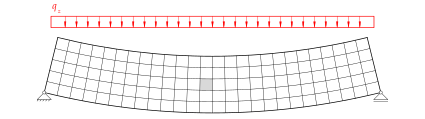
\includegraphics{index_files/mediabag/../images/Kontinua_system.pdf}

}

\caption{\label{fig-reine_biegung_system}Statisches System mit finiten
Elementen}

\end{figure}

Der Vorteil dieser Beziehungen liegt darin, dass diese allgemein für
Biegeprobleme angewendet werden können. Als Gedankenexperiment kann man
sich folgendes vorstellen. Man kann die differentiellen Elemente
beliebig anordnen und weitere statische Systeme zu bilden, die
differentiellen Beziehungen bleiben jedoch die selben.

Die Schnittkräfte am Differentiellen Element sind in
Abbildung~\ref{fig-system_reine_biegung_element} gezeigt. Ebenfalls ist
der verformte Zustand dargstellt, dieser bietet Auskunft über die
kinematischen Relationen.

\begin{figure}[H]

{\centering 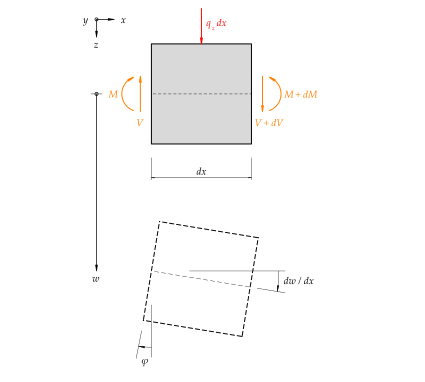
\includegraphics{index_files/mediabag/../images/Kontinua_element.pdf}

}

\caption{\label{fig-system_reine_biegung_element}Differentielles Element
des reinen Beigebalkens}

\end{figure}

Um die Beziehung für den reinen Biegeträger herzuleiten, sind neben den
Gleichgewichtsbedingungen und kinematischen Relationen ebenfalls die
Werkstoffbeziehungen erforderlich.

\hypertarget{herleitung}{%
\subsection{Herleitung}\label{herleitung}}

Beginnend bei den Gleichgewichtsbetrachtungen kann anhand des
Gleichgewichts der vertikalen Kräfte die Beziehung in
Gleichung~\ref{eq-dgl_v_x} zwischen Einwirkung und Querkraft ermittelt
werden:

\[
\downarrow^+\sum F_z = 0 = q_z(x)\cdot dx -V + (V+dV)
\]

\[
q_z(x)\cdot dx = - dV
\]

\begin{equation}\protect\hypertarget{eq-dgl_v_x}{}{
q_z(x) = \frac{dV}{dx} = -V(x)'     
}\label{eq-dgl_v_x}\end{equation}

Aus dem Gleichgewicht der Momente folgt die Gleichung~\ref{eq-dgl_M_y},
welche die Beziehung zwischen Einwirkung und Biegemoment erläutert.

\[
\sum^{\curvearrowleft+} M_y = 0 = (M+dM) - M - V \cdot dx + q_z(x)\cdot dx \cdot dx/2
\]

Dabei kann der Anteil aus der Einwirkung \(q_z(x)\cdot dx \cdot dx/2\)
vernachlässigt werden, da dieser von höherer Ordnung klein ist, es
folgt: \[
0 = dM - V \cdot dx
\]

Umgeformt resultiert die Beziehung zwischen Querkraft und Biegemoment:
\[
V = \frac{dM}{dx} 
\]

Unter Berücksichtigung von Gleichung~\ref{eq-dgl_v_x} folgt die
Gleichung~\ref{eq-dgl_M_y}:
\begin{equation}\protect\hypertarget{eq-dgl_M_y}{}{
q_z(x) = -V(x)'= -M(x)''
}\label{eq-dgl_M_y}\end{equation}

Weitere Beziehungen lassen sich mittels Gleichgewicht nicht ermitteln.
Berücksichtigt man die Werkstoffbeziehungen und kinematischen
Relationen, so lassen sich Aussagen zwischen Einwirkung und Verformung
ermitteln. Um die Herleitung abzukürzen wird die Beziehung in
Gleichung~\ref{eq-momentenkrümmung} zwischen Biegemoment und Krümmung
vorausgesetzt.

\begin{equation}\protect\hypertarget{eq-momentenkruxfcmmung}{}{
\frac{M}{EI} = \chi
}\label{eq-momentenkrümmung}\end{equation}

Allgemein gilt, die Krümmung entspricht der Änderung der Verdrehung:

\begin{equation}\protect\hypertarget{eq-krummung}{}{
\chi = \varphi(x)'
}\label{eq-krummung}\end{equation}

Aus der verformten Lage in
Abbildung~\ref{fig-system_reine_biegung_element}, lässt sich die
Verdrehung des Elements bestimmen. Da das Element seiner Form treu
bleibt, entspricht die Verdrehung der Änderung der Verformung.

\[
-\varphi = \frac{dw}{dx}
\]

Daraus folgt die Beziehung zwischen Biegemoment und Verformung:

\[
M = -EIw(x)''
\]

Unter Berücksichtigung von Gleichung~\ref{eq-dgl_M_y} folgt die
Beziehung zwischen Verformung und Einwirkung.
\begin{equation}\protect\hypertarget{eq-dgl_reine_biegung}{}{
q(x) = EIw(x)''''
}\label{eq-dgl_reine_biegung}\end{equation}

\hypertarget{anwendungen-und-grenzen}{%
\subsection{Anwendungen und Grenzen}\label{anwendungen-und-grenzen}}

Das angewendete Modell berücksichtigt keine Schubverformungen. Da in der
Praxis übliche Stahlbetonbauteile eine signifikant grössere
Schubsteifigkeit, als Biegesteifigkeit aufweisen, liefert das Modell
zuverlässige Resultate. Dazu gelten die Beziehungen lediglich für
konstante Biegesteifigkeiten.

\hypertarget{sec-mohrsche_analogie}{%
\section{Mohrsche Analogie}\label{sec-mohrsche_analogie}}

\hypertarget{aufbau-1}{%
\subsection{Aufbau}\label{aufbau-1}}

Die Mohrsche Analogie beschreibt ein handhabbares Lösungsvorgehen der
Differentialgleichung für reine Biegeträger. Aus den Beziehungen,
detailliert beschrieben in Kapitel~\ref{sec-kontinua}, können folgende
Abhängigkeiten definiert werden:

\[
\frac{d^2M}{dx^2} = M'' = -q_z
\]

\[
\frac{d^2w}{dx^2} = w'' = -\frac{M}{EI}
\]

Erkennbar ist die Analogie der beiden Gleichungen. Aus der Einwirkung
lässt sich der Verlauf der Biegemomente bestimmen. Wird nun auf ein
analoges System der Verlauf der Biegemomente dividiert durch die
Biegesteifigkeit als Einwirkung angesetzt, so lässt sich mit dem
gleichen Berechnungsvorgehen die Verformung bestimmen. Lediglich den
Randbedingungen ist Beachtung zu schenken, welche mit entsprechenden
Lagerungsbedingungen im analogen System berücksichtigt werden.

Die Anpassung der Lagerungsbedingungen für ein analoges System ist in
Abbildung~\ref{fig-randbedingungen_analogiesysteme} gezeigt.

\begin{figure}[H]

{\centering 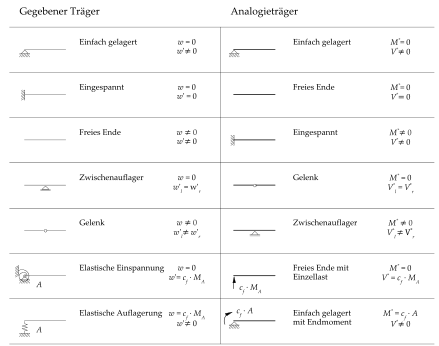
\includegraphics{index_files/mediabag/../images/analogietrager.pdf}

}

\caption{\label{fig-randbedingungen_analogiesysteme}Lagerungsbedingungen
für Analogiesysteme, übernommen aus Spathelf
(\protect\hyperlink{ref-Spathelf2022}{2022})}

\end{figure}

\hypertarget{zuggurtmodell}{%
\section{Zuggurtmodell}\label{zuggurtmodell}}

\hypertarget{aufbau-2}{%
\subsection{Aufbau}\label{aufbau-2}}

Der folgende Abschnitt beschreibt das Zuggurtmodell anhand der
Herleitungen in Spathelf (\protect\hyperlink{ref-Spathelf2022}{2022}).
Das Zuggurtmodell betrachtet auf Zug beanspruchte Stahlbetonzugglieder.
Das Modell erlaubt eine Eingrenzung der Rissbreiten und der
Rissabständen. Im Bereich zwischen den Rissen erhöht sich die
Steifigkeit des Zugglieds, da der Beton sich am Lastabtrag beteiligt.
Dies wird als Zugversteifung beschrieben. Um das Verhalten des Verbunds
zwischen Beton und Betonstahl im ungerissenen Bereich zu definieren,
wird eine Verbundschubspannungs-Schlupfbeziehung dem Modell zu Grunde
gelegt.

\begin{figure}[H]

{\centering 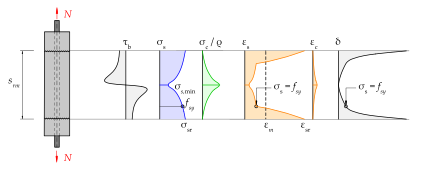
\includegraphics{index_files/mediabag/../images/Zuggurtmodell_grund.pdf}

}

\caption{\label{fig-zuggurtmodell}Verlauf der Verbundschubspannungen,
Betonstahlspannungen, Betonspannungen, Betonstahldehnungen,
Betondehnungen und Schlupf bei einem Zugglied. Bild neu gezeichnet nach
Spathelf (\protect\hyperlink{ref-Spathelf2022}{2022})}

\end{figure}

Verwendet wird eine abegtreppte, starr-ideal plastische
Verbundschubspannungs-Schlupfbeziehung. Durch die Idealisierung lassen
sich die Spannungen und Dehnungen durch Gleichgewichtsbetrachtungen
ermitteln. Die Abtreppung erfolgt beim Erreichen der Fliessgrenze des
Betonstahls.

\begin{figure}[H]

{\centering 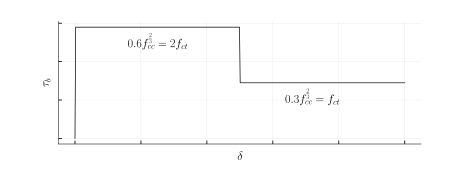
\includegraphics{index_files/mediabag/../images/verbund_schlupf.pdf}

}

\caption{\label{fig-verbund_schlupf}idealisierte
Verbundschubspannungs-Schlupfbeziehung}

\end{figure}

\hypertarget{verhalten-unter-belastung}{%
\subsubsection{Verhalten unter
Belastung}\label{verhalten-unter-belastung}}

Vor dem erreichen der Zugfestigkeit des Betons, verbleibt das Zugglied
ungerissen und verhält sich linear elastisch. Beim Reissen des
Querschnitts verharrt die Betonspannung bei der Rissspannung, eine
Erhöhung der Einwirkung erhöht lediglich die Zugspannung im Betonstahl.

Marti hat in xx ein Ansatz zur Berücksichtigung der Zugversteifung
basierend auf dem Zuggurtmodell für Biegeelemente entwickelt.

\begin{figure}[H]

{\centering 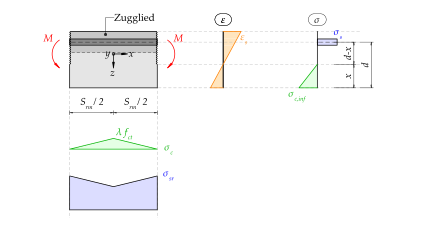
\includegraphics{index_files/mediabag/../images/QS_zugversteifung.pdf}

}

\caption{\label{fig-einfluss_zugversteifung}Einfluss der
Zugversteifenden Wirkung bei einem Biegeelement}

\end{figure}

Vereinfach lässt sich eine Dehnungsreduktion im Betonstahl durch die
Zugversteifung beschreiben, welche mit
\(\Delta \varepsilon_s (\lambda)\) beschrieben wird. Die
Krümmungsdifferenz infolge der Dehnungsreduktion folgt nach
Gleichung~\ref{eq-krummungsdiff}.

\begin{equation}\protect\hypertarget{eq-krummungsdiff}{}{
\Delta \chi(\lambda) = \frac{\Delta \varepsilon_s (\lambda)}{(d-x)} = \frac{\lambda}{2} \cdot \left ( \frac{M_r}{EI^{II}} - \frac{f_{ct}}{E_c\cdot(d-x)}\right )
}\label{eq-krummungsdiff}\end{equation}

Dabei wird die gesamten Krümmung \(\frac{M_r}{EI^{II}}\) beim Reissen
des Querschnitts durch die Krümmung beim Erreichen der Zugfestigkeit des
Betons \(\frac{f_{ct}}{E_c\cdot(d-x)}\) reduziert.

Die Gleichung~\ref{eq-krummungsdiff} kann mittels dem effektiven
Bewehrungsgehalt formuliert werden.

\begin{equation}\protect\hypertarget{eq-rho_eff}{}{
\rho_{\text{eff}} = \left [\frac{M_r(d-x)\cdot E_S}{f_{ct}\cdot EI^{II}}+1-n \right ]^{-1}
}\label{eq-rho_eff}\end{equation}

\[
\Delta \chi(\lambda) = \frac{\lambda}{2} \cdot \frac{f_{ct} \cdot (1-\rho_{\text{eff}})}{\rho_{\text{eff}} \cdot E_s \cdot (d-x)}
\]

Der Beiwert \(\lambda\) dient zur Fallunterscheidung. Grundsätzlich gilt
die Annahme, dass sich ein Riss einstellt beim Erreichen der
Zugfestigkeit des Betons.

\begin{figure}[H]

{\centering 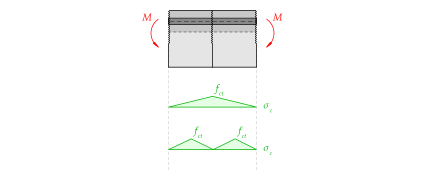
\includegraphics{index_files/mediabag/../images/lambda_beiwert.pdf}

}

\caption{\label{fig-fallunterscheidung_lambda_riss}Fallunterscheidung
beim Erreichen der Zugfestigkeit des Betons}

\end{figure}

Betrachtet man die Darstellung in
Abbildung~\ref{fig-fallunterscheidung_lambda_riss}, so müsste sich in
der Elementmitte ein Riss einstellen. Dabei wird zwischen unmittelbar
vor dem Reissen unterschieden und unmittelbar nach dem Reissen. Dies
kann mit Beiwert unterschieden werden.

\hypertarget{anwendungen-und-grenzen-1}{%
\subsubsection{Anwendungen und
Grenzen}\label{anwendungen-und-grenzen-1}}

Das Zuggurtmodell findet Anwendung Biegebeanspruchungen. Es liefert
Auskunft über Rissweiten und Rissbreiten, sowie eine Verfeinerung der
Biegesteifigkeit im gerissenen Bereich. Das Modell beschränkt sich
ausschliesslich auf normalzugbeanspruchte Bauteile.

\hypertarget{numerische-integration-der-kruxfcmmung}{%
\section{Numerische Integration der
Krümmung}\label{numerische-integration-der-kruxfcmmung}}

\hypertarget{momenten-kruxfcmmungsdiagramm}{%
\subsection{Momenten-Krümmungsdiagramm}\label{momenten-kruxfcmmungsdiagramm}}

Das Momenten-Krümmungsdiagramm ist geeignet zur Beschreibung des
Tragverhaltens von überwiegend auf Biegung beanspruchte Stabtragwerke.
Zur rechnerischen Ermittlung gelten folgende Annahmen, wie in Spathelf
(\protect\hyperlink{ref-Spathelf2022}{2022}) beschrieben:

\begin{itemize}
\tightlist
\item
  Eben- und senkrechtbleiben der Querschnitte
\item
  Die Betonzugfestigkeit \(f_{ct}\) wird, für Zustände nach dem
  Überschreiten von \(f_{ct}\), vernachlässigt
\item
  Linear elastisches Verhalten von Stahl und Beton für die Spannungs-
  und Verformungsberechnung
\item
  Die Bewehrung überträgt Zug- und Druckkräfte ausschliesslich in
  Stabrichtung
\end{itemize}

\hypertarget{versatzmass}{%
\section{Versatzmass}\label{versatzmass}}

\bookmarksetup{startatroot}

\hypertarget{verformung-an-dreipunktbiegeversuch}{%
\chapter{Verformung an
Dreipunktbiegeversuch}\label{verformung-an-dreipunktbiegeversuch}}

Im folgenden Kapitel werden sämtliche Modelle, welche in
Kapitel~\ref{sec-modellbeschrieb} erläutert sind, auf einen
Dreipunktbiegeversuch angewendet. Es wird das Ziel verfolgt, die
Abweichungen der Verformungen, ermittelt mit den unterschiedlichen
Modellen, zu den gemessenen Verformungen darzustellen.

\hypertarget{versuchsbeschrieb}{%
\section{Versuchsbeschrieb}\label{versuchsbeschrieb}}

Es dient der Versuch A3 in der zweiten Versuchsanordnung (kurz A3V2) aus
Jäger und Marti (\protect\hyperlink{ref-Jaeger2006}{2006}). Folgend sind
die notwendigen Eckdaten des Versuchs aufgezeigt, detaillierte
Beschriebe finden sich in Jäger und Marti
(\protect\hyperlink{ref-Jaeger2006}{2006}).

Es handelt sich um einen Plattenstreifen, die Lagerung entspricht einem
Dreipunktbiegeversuch. Belastet wird der Plattenstreifen durch \(F_A\)
bis zum Bruch. Die Höchstlast beträgt \(331 \text{ kN}\).

\begin{figure}[H]

{\centering 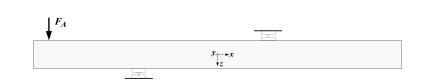
\includegraphics{index_files/mediabag/../images/belastung_a3v2.pdf}

}

\caption{Lagerung und Belastung des Plattenstreifens Versuch A3V2,
entnommen aus Jäger und Marti
(\protect\hyperlink{ref-Jaeger2006}{2006})}

\end{figure}

Das Bewehrungslayout ist so gewählt, dass lediglich eine Zugbewehrung im
negativen Momentenbereich vorhanden ist. Die Bewehrungsrichtung ist
orthogonal, bzw. parallel zu den Bauteilkanten verlegt.

\begin{figure}[H]

{\centering 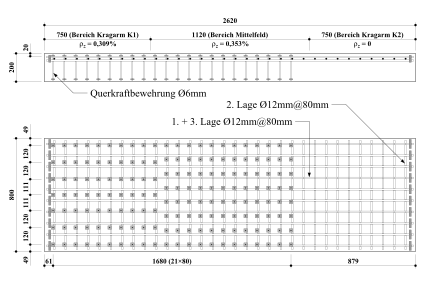
\includegraphics{index_files/mediabag/../images/bewehrung_a3v2.pdf}

}

\caption{Bewehrungslayout des Plattenstreifens Versuch A3V2, entnommen
aus Jäger und Marti (\protect\hyperlink{ref-Jaeger2006}{2006})}

\end{figure}

Die vorhandene Querkraftbewehrung ermöglicht ein weitgehend durch die
Biegung verursachtes Versagen. Dies deckt sich mit der Abgrenzung,
primär Biegeverformungen zu betrachten.

\hypertarget{baustoffeigenschaften}{%
\section{Baustoffeigenschaften}\label{baustoffeigenschaften}}

Mittels Würfel- und Zylinderproben sind Betoneigenschaften in Jäger und
Marti (\protect\hyperlink{ref-Jaeger2006}{2006}) ermittelt worden. Sowie
durch Zugproben die Eigenschaften des Betonstahls. Die
Betoneigenschaften des Würfels decken sich nicht direkt mit den
Eigenschaften des Betons im Bauteil. Mittels Transformationen aus Jaeger
(\protect\hyperlink{ref-Jaeger2014}{2014}) sind die Bauteileigenschaften
bestimmt worden.

Die Betondruckfestigkeit entspricht:

\begin{equation}f_{c} = 2.7 f_{cc}^{\frac{2}{3}}\end{equation}

\begin{equation}f_{c} = \frac{40.827 \text{N}}{\text{mm}^{2}}\end{equation}

Zugfestigkeit nach Jaeger (\protect\hyperlink{ref-Jaeger2013}{2013}):

\begin{equation}f_{ct} = 0.3 f_{cc}^{\frac{2}{3}}\end{equation}

\begin{equation}f_{ct} = \frac{4.54 \text{N}}{\text{mm}^{2}}\end{equation}

Elastizitätsmodul nach Jaeger
(\protect\hyperlink{ref-Jaeger2013}{2013}):

\begin{equation}E_{c} = 10000 \sqrt[3]{f_{cc}}\end{equation}

\begin{equation}E_{c} = \frac{38886.0 \text{N}}{\text{mm}^{2}}\end{equation}

\hypertarget{reiner-biegetruxe4ger}{%
\section{Reiner Biegeträger}\label{reiner-biegetruxe4ger}}

In diesem Abschnitt wird das Modell aus Kapitel~\ref{sec-kontinua} auf
das Versuchsobjekt angewendet. Dazu ist in einem ersten Schritt das
statische System des Versuchs in Abbildung~\ref{fig-system_2}
aufgezeigt.

\begin{figure}[H]

{\centering 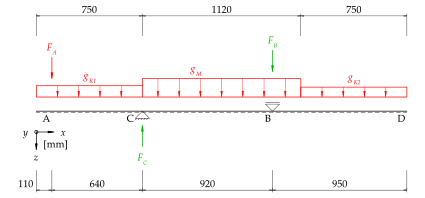
\includegraphics{index_files/mediabag/../images/System_anordnung_2.pdf}

}

\caption{\label{fig-system_2}Statisches System der Versuchsanordnung}

\end{figure}

Eine Vereinfachung des Systems in Abbildung~\ref{fig-system_2} ist in
Abbildung~\ref{fig-system_2_lager} gezeigt. Dabei wird das Eigengewicht
vernachlässigt, aufgrund des minimalen Einflusses des Eigengewichts auf
das Biegemoment. Sowie sind die Verformungen, gemessen in Jäger und
Marti (\protect\hyperlink{ref-Jaeger2006}{2006}), nach dem Einbau des
Trägers gemessen worden. Folglich zeigt die Messung den Einfluss des
Eigengewichts nicht.

\begin{equation}\protect\hypertarget{eq-eigengewicht}{}{
g_M, g_{k1}, g_{k2} = 0
}\label{eq-eigengewicht}\end{equation}

Die Berücksichtigung der Lagerbreiten führt zu der Streckenlast \(f_A\),
bzw. zu den Lagerreaktionen \(f_B\) und \(f_C\).

\begin{figure}[H]

{\centering 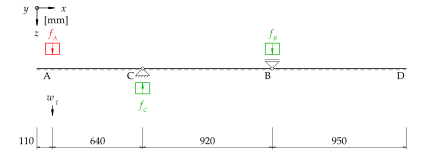
\includegraphics{index_files/mediabag/../images/System_anordnung_2_lagerbreite.pdf}

}

\caption{\label{fig-system_2_lager}Angepasstes statisches System der
Versuchsanordnung}

\end{figure}

Die Berechnungen beziehen sich ausschliesslich auf
Abbildung~\ref{fig-system_2_lager}. Dazu sind die folgenden Parameter
berücksichtigt:

\hypertarget{tbl-params_reiner_biegetraeger}{}
\begin{longtable}[]{@{}
  >{\raggedright\arraybackslash}p{(\columnwidth - 2\tabcolsep) * \real{0.5000}}
  >{\raggedright\arraybackslash}p{(\columnwidth - 2\tabcolsep) * \real{0.5000}}@{}}
\caption{\label{tbl-params_reiner_biegetraeger}Versuchsparameter für den
reinen Biegeträger}\tabularnewline
\toprule\noalign{}
\endfirsthead
\endhead
\bottomrule\noalign{}
\endlastfoot
\(a_{1} = 0.11 \, \text{m}\) & \(a_{2} = 0.64 \, \text{m}\) \\
\(a_{3} = 0.92 \, \text{m}\) & \(a_{4} = 0.95 \, \text{m}\) \\
\(b = 800.0 \, \text{mm}\) & \(b_{Auflager} = 100 \, \text{mm}\) \\
\(h = 200.0 \, \text{mm}\) & \\
\end{longtable}

\hypertarget{auflagerkruxe4fte}{%
\subsection{Auflagerkräfte}\label{auflagerkruxe4fte}}

Anhand von Gleichgewichtsbeziehungen können für das statisch bestimmte
System die Auflagerkräfte bestimmt werden. In einem ersten Schritt wird
die Balkenlänge definiert:

\begin{equation}l_{tot} = a_{1} + a_{2} + a_{3} + a_{4}\end{equation}

\begin{equation}l_{tot} = 2.62 \text{m}\end{equation}

Durch Momentengleichgewicht um die Auflagerpunkte \(C\) und \(B\) folgen
die Beziehungen zwischen Einwirkung und Reaktionskräfte:

\begin{equation}0 = F_{A} a_{2} - F_{B} a_{3}\end{equation}

\begin{equation}0 = F_{A} \left(a_{2} + a_{3}\right) - F_{C} a_{3}\end{equation}

Durch Auflösung nach den Reaktionskräften folgt:

\begin{equation}F_{B} = \frac{F_{A} a_{2}}{a_{3}}\end{equation}

\begin{equation}F_{C} = \frac{F_{A} a_{2} + F_{A} a_{3}}{a_{3}}\end{equation}

Wie in Abbildung~\ref{fig-system_2_lager} gezeigt, gilt es die
Punktkräfte der Auflagerbreite entsprechend zu verteilen:

\begin{equation}f_{B} = \frac{F_{A} a_{2}}{a_{3} b_{Auflager}}\end{equation}

\begin{equation}f_{C} = \frac{F_{A} a_{2} + F_{A} a_{3}}{a_{3} b_{Auflager}}\end{equation}

\begin{equation}f_{A} = \frac{F_{A}}{b_{Auflager}}\end{equation}

\hypertarget{zustandslinien}{%
\subsection{Zustandslinien}\label{zustandslinien}}

Die Zustandslinien der Schnittkräfte resultieren aus der Bemühung der
hergeleiteten Gleichungen in Kapitel~\ref{sec-kontinua}. Dabei ist zu
beachten, dass die Zustandslinien lediglich für die maximal gewählte
Laststufe gelten. Der Verlauf der Einwirkungen ist in
Abbildung~\ref{fig-q_x} aufgezeigt. Es sind lediglich die bestimmten
Einwirkungen und Reaktionen an den Stab anzusetzen. Die positive
Stabseite ist strichliert dargestellt. In positive z-Richtung wirkende
Kräfte sind positiv definiert.

\begin{figure}[H]

{\centering 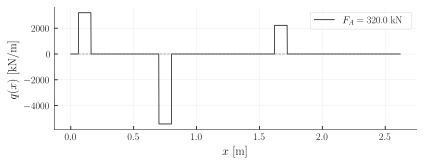
\includegraphics{index_files/mediabag/06_Versuch_2_A3_Jaeger_files/figure-pdf/fig-q_x-output-1.pdf}

}

\caption{\label{fig-q_x}Verlauf der Einwirkungen und Reaktionskräften}

\end{figure}

Durch Integration der Einwirkung resultiert der Querkraftverlauf.

\begin{equation}\protect\hypertarget{eq-vx_integriert}{}{
V(x) = -\int q(x) + c_1
}\label{eq-vx_integriert}\end{equation}

Dabei kann mit der Randbedingun \(V(0) = 0\) die Integrationskonstante
ermittelt werden. Der Verlauf der Querkräfte ist in
Abbildung~\ref{fig-v_x} dargestellt. Nach dem Auflager \(B\) ist der
Plattenstreifen unbelastet.

\begin{figure}[H]

{\centering 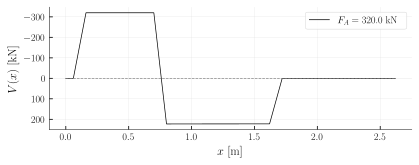
\includegraphics{index_files/mediabag/06_Versuch_2_A3_Jaeger_files/figure-pdf/fig-v_x-output-1.pdf}

}

\caption{\label{fig-v_x}Verlauf der Querkräfte}

\end{figure}

Der Verlauf der Biegemoment lässt sich durch Integration der Querkräfte
bestimmen:

\[
M(x) = \int V(x) + c_2
\]

Dabei kann mit der Randbedingung \(M(0) = 0\) die Integrationskonstante
ermittelt werden. Der Verlauf der Biegemomente ist in
Abbildung~\ref{fig-m_x} dargestellt. Es stellt sich ein Minimum über dem
Auflager \(C\) ein.

\begin{figure}[H]

{\centering 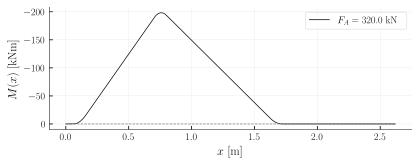
\includegraphics{index_files/mediabag/06_Versuch_2_A3_Jaeger_files/figure-pdf/fig-m_x-output-1.pdf}

}

\caption{\label{fig-m_x}Verlauf der Biegemomente}

\end{figure}

Neben den resultierenden Biegemomenten aus der Einwirkung kann ein
Biegemoment, induziert durch die Längszukraft aus der Querkraft,
ermittelt werden. Dies ist mit einem Versatzmass berücksichtigt. Dabei
gilt das Versatzmass lediglich für die Längszugkraft. Multipliziert mit
der statischen Höhe resultiert der Versatz des Biegemoments

\begin{equation}\protect\hypertarget{eq-versatzmass}{}{
h_{versatz} = \frac{V \cdot \cot(\theta_{c3})}{2}
}\label{eq-versatzmass}\end{equation}

\begin{equation}\protect\hypertarget{eq-versatzmment}{}{
M_{versatz} = \frac{V \cdot \cot(\theta_{c3})}{2} \cdot z
}\label{eq-versatzmment}\end{equation}

Der Momentenverlauf in Abbildung~\ref{fig-m_x} ist mit dem Versatzmass
zu erhöhen. Dargestellt ist dies in Abbildung~\ref{fig-m_x_versatz}.
Beim Momentenminimum bildet sich ein Plateau aus.

\begin{figure}[H]

{\centering 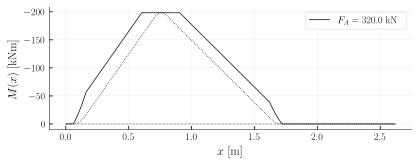
\includegraphics{index_files/mediabag/06_Versuch_2_A3_Jaeger_files/figure-pdf/fig-m_x_versatz-output-1.pdf}

}

\caption{\label{fig-m_x_versatz}Verlauf der Biegemomente mit
Längszugkraft aus Querkraft}

\end{figure}

\hypertarget{biegesteifigkeit---vollstuxe4ndig-ungerissen}{%
\subsubsection{Biegesteifigkeit - Vollständig
ungerissen}\label{biegesteifigkeit---vollstuxe4ndig-ungerissen}}

Wie in Kapitel~\ref{sec-kontinua} hergeleitet, sind die
Gleichgewichtsbetrachtungen nicht ausreichend um die Verdrehung und
Verformung zu beschreiben. Die Werkstoffbeziehung bedingt eine
Biegesteifigkeit. Dabei wird von einer konstanten Biegesteifigkeit
ausgegangen. Für einen ungerissenen Querschnitts folgt diese zu:

\begin{equation}EI = \frac{E_{c} b h^{3}}{12}\end{equation}

\begin{equation}EI = 2.07 \cdot 10^{4} \text{kN} \text{m}^{2}\end{equation}

Der Verlauf der Verdrehung entspricht dem Integrierten Verlauf der
Biegemomente, dividiert durch die Biegesteifigkeit.

\begin{equation}\protect\hypertarget{eq-verdrehung}{}{
\varphi(x) = \frac{1}{EI}\int M(x) + c_3
}\label{eq-verdrehung}\end{equation}

Abschliessend lässt sich die Verformung anhand der Verdrehung ermitteln.

\begin{equation}\protect\hypertarget{eq-verformung}{}{
w(x) = \int -\varphi(x) + c_4
}\label{eq-verformung}\end{equation}

Mit den Randbedingungen \(w(C) = 0\) und \(w(B) = 0\) sind die
Integrationskonstanten bestimmt. Die elastische Verformung für einen
ungerissenen Querschnitt ist in Abbildung~\ref{fig-w_x} dargestellt.

\begin{figure}[H]

{\centering 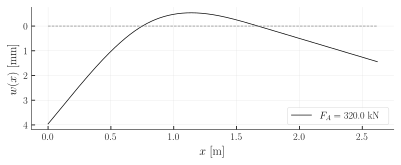
\includegraphics{index_files/mediabag/06_Versuch_2_A3_Jaeger_files/figure-pdf/fig-w_x-output-1.pdf}

}

\caption{\label{fig-w_x}Verlauf der Verformung für eine konstante
ungerissene Biegesteifigkeit}

\end{figure}

\hypertarget{mohrsche-analogie}{%
\section{Mohrsche Analogie}\label{mohrsche-analogie}}

Das Vorgehen ist in Kapitel~\ref{sec-mohrsche_analogie} beschrieben. Der
bereits bestimmte Momentenverlauf gemäss Abbildung~\ref{fig-m_x},
dividiert durch die ungerissene Biegesteifigkeit, ist als Einwirkung auf
das System anzusetzen. Dargestellt ist dies in
Abbildung~\ref{fig-q_x_mohr}.

\begin{figure}[H]

{\centering 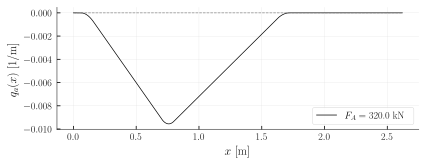
\includegraphics{index_files/mediabag/06_Versuch_2_A3_Jaeger_files/figure-pdf/fig-q_x_mohr-output-1.pdf}

}

\caption{\label{fig-q_x_mohr}Verlauf der Einwirkungen auf das analoge
System}

\end{figure}

Die maximale Biegeverformung tritt beim Stabanfang auf. Gemäss der
Abbildung~\ref{fig-w_x} ist bekannt, dass bei den Auflagerpunkten die
Verformung gleich null sein muss, sowie die Verformung am Stabanfang und
einen Maximalwert aufweist. Die Verformung bei der Mohrschen Analogie
entspricht dem Biegemomentenverlauf des analogen Systems. Folglich ist
bei den Stab Anfangs- und Endpunkten eine volle Einspannung zu
modellieren, sowie bei den Auflagerpunkten ein Biegegelenk einzuführen.
Dies deckt sich mit den Lagerungsbedingungen aus
Abbildung~\ref{fig-randbedingungen_analogiesysteme}.

\begin{figure}[H]

{\centering 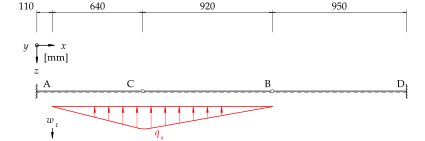
\includegraphics{index_files/mediabag/../images/System_analog.pdf}

}

\caption{\label{fig-system_analog}Analoges System mit entsprechender
Einwirkung und Lagerungsbedingungen}

\end{figure}

Der Querkraftverlauf für das analoge Sytem ist in
Abbildung~\ref{fig-v_x_mohr} aufgezeigt. Die Querkraft ist einheitslos,
da es sich um die Verdrehung handelt.

\begin{figure}[H]

{\centering 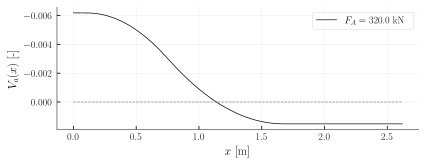
\includegraphics{index_files/mediabag/06_Versuch_2_A3_Jaeger_files/figure-pdf/fig-v_x_mohr-output-1.pdf}

}

\caption{\label{fig-v_x_mohr}Verlauf der Querkräfte für das
Analogiesystem}

\end{figure}

Der Biegemomentenverlauf für das analoge System zeigt die
Abbildung~\ref{fig-m_x_mohr}. Der Momentenverlauf entspricht der
Verformung und ist folglich in {[}mm{]} dargestellt.

\begin{figure}[H]

{\centering 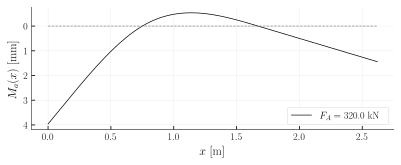
\includegraphics{index_files/mediabag/06_Versuch_2_A3_Jaeger_files/figure-pdf/fig-m_x_mohr-output-1.pdf}

}

\caption{\label{fig-m_x_mohr}Verlauf der Biegemomente für das
Analogiesystem}

\end{figure}

\hypertarget{abschuxe4tzung-nach-norm}{%
\section{Abschätzung nach Norm}\label{abschuxe4tzung-nach-norm}}

Nach der bestimmten elastischen Verformung kann die Verformung anhand
des vollständig gerissenen Querschnitts nach SIA
(\protect\hyperlink{ref-SIA2013a}{2013}) ermittelt werden. Ohne
Druckbewehrung und Kriecheinflüsse folgt die Gleichung zu:

\begin{equation}\protect\hypertarget{eq-w_1_II_sia}{}{
w_{1II,SIA} = \frac{0.75}{10\rho^{0.7}}\left(\frac{h}{d}\right)^3 w_1
}\label{eq-w_1_II_sia}\end{equation}

Dabei entspricht der geometrische Bewehrungsgehalt:

\begin{equation}\rho = \frac{A_{s}}{b d}\end{equation}

Die Querschnittsfläche der Stäbe folgt zu:

\begin{equation}A_{s} = 2 b \frac{\pi \oslash_{s}^{2}}{4 s_{x}}\end{equation}

\begin{equation}A_{s} = 2262.0 \text{mm}^{2}\end{equation}

Die statische Höhe ist definiert gemäss:

\begin{equation}d = - \frac{3 \oslash_{s}}{2} - c_{nom} + h\end{equation}

\begin{equation}d = 162.0 \text{mm}\end{equation}

Die Verformung entspricht abschliessend:

\begin{equation}w_{1 II,SIA} = 15.7 \text{mm}\end{equation}

\hypertarget{numerische-integration-der-kruxfcmmung-1}{%
\section{Numerische Integration der
Krümmung}\label{numerische-integration-der-kruxfcmmung-1}}

\hypertarget{grundlagen}{%
\subsection{Grundlagen}\label{grundlagen}}

Um sich von der Betrachtung einer konstanten Biegesteifigkeit zu lösen,
hilft die Anwendung einer verfeinerten Momenten-Krümmungsbeziehung.
Folgend wird ein Momentenkrümmungsdiagramm für den Querschnitt aus dem
beschriebenen Versuch berechnet. Die vorhandene Querkraftbewehrung ist
nicht dargestellt in Abbildung~\ref{fig-qs_a3}.

\begin{figure}[H]

{\centering 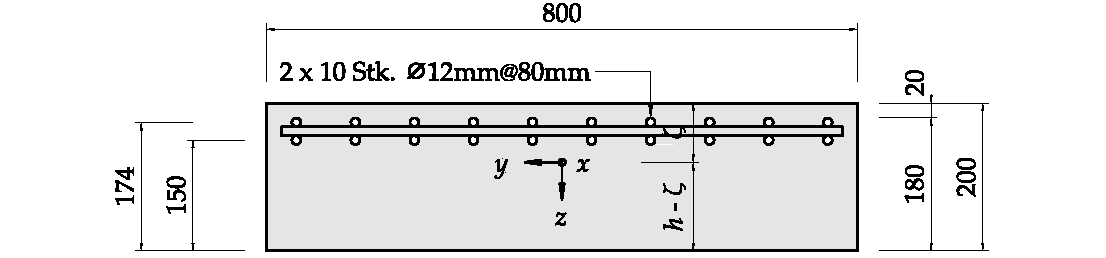
\includegraphics{index_files/mediabag/../images/QS_Versuch_A3.pdf}

}

\caption{\label{fig-qs_a3}Querschnitt des Versuchs A3 zur Bestimmung des
Momenten-Krümmungdiagramms}

\end{figure}

Vereinfacht wird der Querschnitt folgender massen:

\begin{figure}[H]

{\centering 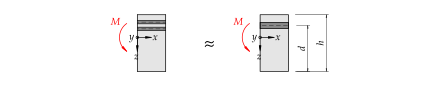
\includegraphics{index_files/mediabag/../images/QS_analyse_1.pdf}

}

\caption{Vereinfachung der Bewehrungsführung}

\end{figure}

Die Parameter in Tabelle~\ref{tbl-params_krummung} finden Einfluss in
die Berechnungen.

\hypertarget{tbl-params_krummung}{}
\begin{longtable}[]{@{}
  >{\raggedright\arraybackslash}p{(\columnwidth - 2\tabcolsep) * \real{0.5000}}
  >{\raggedright\arraybackslash}p{(\columnwidth - 2\tabcolsep) * \real{0.5000}}@{}}
\caption{\label{tbl-params_krummung}Versuchsparameter für die
verfeinerte Momenten-Krümmungsbeziehung}\tabularnewline
\toprule\noalign{}
\endfirsthead
\endhead
\bottomrule\noalign{}
\endlastfoot
\(E_{s} = 200000.0 \, \frac{\text{N}}{\text{mm}^{2}}\) &
\(\oslash_{s} = 12.0 \, \text{mm}\) \\
\(c_{nom} = 20.0 \, \text{mm}\) &
\(f_{cc} = 58.8 \, \frac{\text{N}}{\text{mm}^{2}}\) \\
\(f_{su} = 630.3 \, \frac{\text{N}}{\text{mm}^{2}}\) &
\(f_{sy} = 546.0 \, \frac{\text{N}}{\text{mm}^{2}}\) \\
\(s_{x} = 80.0 \, \text{mm}\) & \(\varepsilon_{cu} = 0.005\) \\
\(\varepsilon_{su} = 0.1117\) & \\
\end{longtable}

Neben den Parametern wird das Stoffgesetz für den Betonstahl in
Abbildung~\ref{fig-stahlkennlinie} hinterlegt. Das Bilineare, bzw.
linear-elastisch linear-plastische Spannungs-Dehnungsdiagramm für den
Betonstahl hält den Rechenaufwand klein und liefert eine ausreichende
Genauigkeit. Eine Berücksichtigung des verfestigenden Verhaltens ist
essentiell um die Verformungen nach dem Fliessen des Betonstahls
näherungsweise zu bestimmen. Das Diagramm ist definiert bis zur
Bruchdehnung des Stahls. Das Verhalten gilt ebenso im negativen
Spannungs-Dehnungs Bereich.

\begin{figure}[H]

{\centering \includegraphics{index_files/mediabag/06_Versuch_2_A3_Jaeger_files/figure-pdf/fig-stahlkennlinie-output-1.pdf}

}

\caption{\label{fig-stahlkennlinie}Spannungs-Dehnungs Diagramm des
Bewehrungsstahls linear elastisch-linear verfestigend plastisch}

\end{figure}

Die Betonkennlinie in Abbildung~\ref{fig-betonkennlinie} zeigt ein
linear-elastisches ideal-plastisches verhalten. Im positiven Bereich
lässt sich die Betonspannung bis zur Betonzugfestigkeit erhöhen, im
negativen Spannungsbereich beginnt ein Plastifizieren beim Erreichen der
Betondruckfestigkeit. Bis zur Bruchstauchung ist dies definiert.

\begin{figure}[H]

{\centering \includegraphics{index_files/mediabag/06_Versuch_2_A3_Jaeger_files/figure-pdf/fig-betonkennlinie-output-1.pdf}

}

\caption{\label{fig-betonkennlinie}Spannungs-Dehnungs Diagramm des
Betons linear elastisch-ideal plastisch}

\end{figure}

\hypertarget{querschnittsanalyse}{%
\subsection{Querschnittsanalyse}\label{querschnittsanalyse}}

Mittels einer Querschnittsanalyse lassen sich die unterschiedlichen
Zustände des Momenten-Krümmungdiagramms ermitteln.

\hypertarget{schwerpunkt-des-querschnitts}{%
\subsubsection{Schwerpunkt des
Querschnitts}\label{schwerpunkt-des-querschnitts}}

Durch die Bestimmung der Wertigkeit \(n\) kann der Querschnitt als
homogener Betonquerschnitt zur Bestimmung des Schwerpunkts behandelt
werden.

\begin{equation}n = \frac{E_{s}}{E_{c}}\end{equation}

\begin{equation}n = 5.14\end{equation}

Die Querschnittsfläche der Bewehrung beträgt:

\begin{equation}A_{s} = 2 b \frac{\pi \oslash_{s}^{2}}{4 s_{x}}\end{equation}

\begin{equation}A_{s} = 2262.0 \text{mm}^{2}\end{equation}

Die Betonquerschnittsfläche:

\begin{equation}A_{c} = b h\end{equation}

\begin{equation}A_{c} = 160000.0 \text{mm}^{2}\end{equation}

Die ideelle Querschnittsfläche resultiert zu:

\begin{equation}A_{i} = A_{c} + A_{s} \left(n - 1\right)\end{equation}

\begin{equation}A_{i} = 169372.0 \text{mm}^{2}\end{equation}

Und die z-Koordinate des Schwerpunkts folgt abschliessend zu:

\begin{equation}\zeta_{c} = \frac{\frac{A_{c} h}{2} + A_{s} \left(1.5 \oslash_{s} + c_{nom}\right) \left(n - 1\right)}{A_{i}}\end{equation}

\begin{equation}\zeta_{c} = 96.6 \text{mm}\end{equation}

\begin{equation}A_{s} = 22.6 \text{cm}^{2}\end{equation}

\hypertarget{fluxe4chentruxe4gheitsmoment}{%
\subsubsection{Flächenträgheitsmoment}\label{fluxe4chentruxe4gheitsmoment}}

Das Flächenträgheitsmoment wird ebenfalls am ideellen Querschnitt
bestimmt. Die Eigenträgheitsmomente der Kreisquerschnitte der Bewehrung
sind nicht berücksichtigt, lediglich der Steiner-Anteil fliesst in die
Berechnung ein:

\begin{equation}I^{I} = A_{s} \left(n - 1\right) \left(\frac{3 \oslash_{s}}{2} + c_{nom} - \zeta_{c}\right)^{2} + \frac{b h^{3}}{12} + b h \left(\frac{h}{2} - \zeta_{c}\right)^{2}\end{equation}

\begin{equation}I^{I} = 5.67 \cdot 10^{8} \text{mm}^{4}\end{equation}

\hypertarget{ungerissen---zustand-1}{%
\subsubsection{Ungerissen - Zustand 1}\label{ungerissen---zustand-1}}

Der Querschnitt verbleibt elastisch. Folglich kann das
Flächenträgheitsmoment mit \(E_c\) multipliziert werden und es
resultiert die ungerissene Biegesteifigkeit:

\begin{equation}EI^{I} = E_{c} I^{I}\end{equation}

\begin{equation}EI^{I} = 2.206 \cdot 10^{4} \text{kN} \text{m}^{2}\end{equation}

\hypertarget{rissmoment}{%
\paragraph{Rissmoment}\label{rissmoment}}

Durch die Ermittlung des Rissmoments kann die Krümmung vor dem Reissen
des Betons ermittelt werden. Die Betonzugkraft wird nicht
berücksichtigt.

\begin{figure}[H]

{\centering 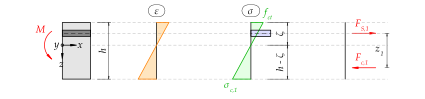
\includegraphics{index_files/mediabag/../images/QS_analyse_2.pdf}

}

\caption{\label{fig-qs2}Querschnittsanalyse vor dem Reissen des Betons}

\end{figure}

Die Betondruckspannung beträgt:

\begin{equation}\sigma_{c inf,1} = \frac{f_{ct} \left(h - \zeta_{c}\right)}{\zeta_{c}}\end{equation}

\begin{equation}\sigma_{c inf,1} = \frac{4.86 \text{N}}{\text{mm}^{2}}\end{equation}

Der Hebelarm der inneren Kräfte folgt zu:

\begin{equation}z_{1} = - 1.5 \oslash_{s} - c_{nom} + \frac{2 h}{3} + \frac{\zeta_{c}}{3}\end{equation}

\begin{equation}z_{1} = 128.0 \text{mm}\end{equation}

Die Betondruckkraft ist definiert nach:

\begin{equation}F_{c,1} = \frac{b \sigma_{c inf,1} \left(h - \zeta_{c}\right)}{2}\end{equation}

\begin{equation}F_{c,1} = 201.0 \text{kN}\end{equation}

Und das Rissmoment resultiert schliesslich zu:

\begin{equation}M_{r} = F_{c,1} z_{1}\end{equation}

\begin{equation}M_{r} = 25.63 \text{kN} \text{m}\end{equation}

Aus dem Rissmoment folgt die Krümmung beim Reissen:

\begin{equation}\chi_{r} = \frac{M_{r}}{EI^{I}}\end{equation}

\begin{equation}\chi_{r} = \frac{0.00116}{\text{m}}\end{equation}

Die Neigung linearen Funktion des ungerissenen Zustands im
Momentenkrümmungsdiagramm ist durch die Biegesteifigkeit definiert. Der
Endpunkts des Zustand 1 definiert das Rissmoment mit der entsprechenden
Krümmung.

\hypertarget{gerissen-elastisch---zustand-2}{%
\subsubsection{Gerissen Elastisch - Zustand
2}\label{gerissen-elastisch---zustand-2}}

Der Querschnitt nach dem Reissen ist in Abbildung~\ref{fig-qs3}
dargestellt. Der Betonstahl hat die Fliessgrenze noch nicht erreicht.
Der Beton die Druckfestigkeit ebenfalls nicht.

\begin{figure}[H]

{\centering 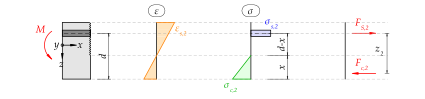
\includegraphics{index_files/mediabag/../images/QS_analyse_3.pdf}

}

\caption{\label{fig-qs3}Querschnittsanalyse nach dem Reissen des Betons}

\end{figure}

Dabei beträgt die statische Höhe:

\begin{equation}d = - \frac{3 \oslash_{s}}{2} - c_{nom} + h\end{equation}

\begin{equation}d = 162.0 \text{mm}\end{equation}

Mittels Gleichgewicht der Kräfte lässt sich die Betondruckzonenhöhe und
folglich die gerissene Biegesteifigkeit herleiten. Die
Betonstahlzugkraft beträgt:

\begin{equation}F_{z,2} = A_{s} \sigma_{s,2}\end{equation}

Die Betonstahlspannung für linear elastisches Verhalten folgt zu:

\begin{equation}\sigma_{s,2} = E_{s} \varepsilon_{s,2}\end{equation}

Die Betondruckkraft anhand des dreieckigen Verlaufs in
Abbildung~\ref{fig-qs3} beträgt:

\begin{equation}F_{c,2} = \frac{b \sigma_{c inf,2} x_{2}}{2}\end{equation}

Die Betonspannung ebenfalls bestimmt durch ein linear elastisches
Verhalten ist definiert durch:

\begin{equation}\sigma_{c inf,2} = E_{c} \varepsilon_{c,2}\end{equation}

Die Betondehnung anhand des Dehnungsverlaufs in Abbildung~\ref{fig-qs3}:

\begin{equation}\varepsilon_{c,2} = \frac{\varepsilon_{s,2} x_{2}}{d - x_{2}}\end{equation}

Unter Bemühung des Gleichgewichts der horizontalen Kräfte lässt sich die
folgende Beziehung ermitteln.

\begin{equation}F_{c,2} = F_{z,2}\end{equation}

Einsetzen der bestimmten Gleichungen in die Gleichgewichtsbeziehung und
mit \(n\) und \(\rho\) substituiert, folgt:

\begin{equation}n = \frac{E_{s}}{E_{c}}\end{equation}

\begin{equation}\rho = \frac{A_{s}}{b d}\end{equation}

\begin{equation}E_{s} b d \rho \varepsilon_{s,2} = \frac{E_{s} b \varepsilon_{s,2} x_{2}^{2}}{2 n \left(d - x_{2}\right)}\end{equation}

Durch die Auflösung nach \(x\) folgt die Betondruckzonenhöhe:

\begin{equation}x_{2} = d \left(- n \rho + \sqrt{n \rho \left(n \rho + 2\right)}\right)\end{equation}

\begin{equation}x_{2} = 55.6 \text{mm}\end{equation}

Zur Bestimmung der Krümmung ist die Betonstahldehnung erforderlich.
Diese bedingt ein einwirkendes Moment. Der Übergang zwischen
ungerissenem zu gerissenem Verhalten erfolgt beim Rissmoment. Folglich
kann das Rissmoment in Abbildung~\ref{fig-qs3} angesetzt werden.

\begin{equation}M_{2} = F_{z,2} \left(d - \frac{x_{2}}{3}\right)\end{equation}

\begin{equation}M_{2} = M_{r}\end{equation}

\begin{equation}M_{r} = A_{s} E_{s} \varepsilon_{s,2} \left(d - \frac{x_{2}}{3}\right)\end{equation}

Daraus resultiert die Betonstahldehnung:

\begin{equation}\varepsilon_{s,2} = 0.000395\end{equation}

Die Krümmung kann anhand des Dehnungsverlaufs in Abbildung~\ref{fig-qs3}
bestimmt werden:

\begin{equation}\chi^{II} = \frac{\varepsilon_{s,2}}{d - x_{2}}\end{equation}

\begin{equation}\chi^{II} = \frac{0.00371}{\text{m}}\end{equation}

Abschliessend folgt die gerissene Biegesteifigkeit zu:

\begin{equation}EI^{II} = \frac{M_{2}}{\chi^{II}}\end{equation}

\begin{equation}EI^{II} = 6903.8 \text{kN} \text{m}^{2}\end{equation}

Die Neigung der linearen Funktion im gerissenen Bereich ist durch die
gerissene Biegesteifigkeit definiert. Der Beginn ist durch das
Rissmoment definiert.

\hypertarget{fliessen-der-bewehrung---zustand-3}{%
\subsubsection{Fliessen der Bewehrung - Zustand
3}\label{fliessen-der-bewehrung---zustand-3}}

Die Biegesteifigkeit \(EI^{II}\) gilt bis die Bewehrung fliesst oder der
Beton beginnt zu plastifizieren. In Abbildung~\ref{fig-qs4} wird
vorausgesetzt, dass die Bewehrung fliesst.

\begin{figure}[H]

{\centering 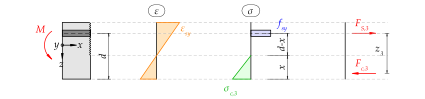
\includegraphics{index_files/mediabag/../images/QS_analyse_4.pdf}

}

\caption{\label{fig-qs4}Querschnittsanalyse für reine Biegung beim
Fliessen der Bewehrung}

\end{figure}

Durch Gleichgewicht der horizontalen Kräfte folgen die Beziehungen:

\begin{equation}\sigma_{c inf,3} = \frac{E_{c} f_{sy} x_{3}}{E_{s} \left(d - x_{3}\right)}\end{equation}

\begin{equation}A_{s} f_{sy} = \frac{b \sigma_{c inf,3} x_{3}}{2}\end{equation}

Aufgelöst nach der Druckzonenhöhe:

\begin{equation}x_{3} = \frac{- A_{s} E_{s} + \sqrt{A_{s} E_{s} \left(A_{s} E_{s} + 2 E_{c} b d\right)}}{E_{c} b}\end{equation}

\begin{equation}x_{3} = 55.6 \text{mm}\end{equation}

Daraus lässt sich das Fliessmoment bestimmen, welches den Endpunkt im
Momenten-Krümmungsdiagramm für den gerissenen Zustand definiert:

\begin{equation}M_{y} = A_{s} f_{sy} \left(d - \frac{x_{3}}{3}\right)\end{equation}

\begin{equation}M_{y} = 177.2 \text{kN} \text{m}\end{equation}

Die Fliessdehnung des Betonstahls entspricht:

\begin{equation}\varepsilon_{sy} = 0.00273\end{equation}

Abschliessend lässt sich die Krümmung für den Endpunkt des Zustands 2
folgend bestimmen:

\begin{equation}\chi_{y} = \frac{\varepsilon_{sy}}{d - x_{3}}\end{equation}

\begin{equation}\chi_{y} = \frac{0.0257}{\text{m}}\end{equation}

Der Zustand 3 beschreibt lediglich den Endpunkt des gerissenen Bereichs
im Momenten-Krümmungsdiagramm.

\hypertarget{maximaler-biegewiderstand---zustand-4}{%
\subsubsection{Maximaler Biegewiderstand - Zustand
4}\label{maximaler-biegewiderstand---zustand-4}}

Abschliessen kann der maximale Biegewiderstand durch die plastifizierung
der Betondruckzone bestimmt werden. Vereinfacht wird dem Betonstahl die
statische Zugfestigkeit vorausgesetzt um das verfestigende Verhalten
annähernd abzubilden. Dies bedingt grundsätzlich das Erreichen der
Bruchdehnung im Stahl. Da der Querschnitt stark bewehrt ist, versagt die
Betondruckzone vor dem Erreichen der Betonstahlbruchdehnung.

\begin{figure}[H]

{\centering 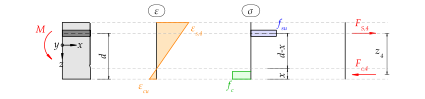
\includegraphics{index_files/mediabag/../images/QS_analyse_5.pdf}

}

\caption{\label{fig-qs5}Querschnittsanalyse für reine Biegung mit der
Bewehrung bei der Bruchspannung und plastifizierter Betondruckzone}

\end{figure}

Vereinfacht werden die Spannungen in der Druckzone konstant verteilt
betrachtet. Dazu wird die Druckzonenhöhe abgemindert um Faktor 0.85.

Das Gleichgewicht der Kräfte führt zu:

\begin{equation}A_{s} f_{su} = 0.85 b f_{c} x_{4}\end{equation}

Die Druckzonenhöhe folgt zu:

\begin{equation}x_{4} = 51.4 \text{mm}\end{equation}

Der maximale Biegewiderstand folgt zu:

\begin{equation}M_{R} = A_{s} f_{su} \left(d - 0.425 x_{4}\right)\end{equation}

\begin{equation}M_{R} = 199.8 \text{kN} \text{m}\end{equation}

Die Krümmung lässt sich anhand der Betonstauchung ermitteln:

\begin{equation}\chi_{u} = \frac{\varepsilon_{cu}}{x_{4}}\end{equation}

\begin{equation}\chi_{u} = \frac{0.0974}{\text{m}}\end{equation}

Die Betonstahldehnung darf die Bruchdehnung nicht überschreiten:

\begin{equation}\varepsilon_{s,4} = \frac{\varepsilon_{cu} \left(d - x_{4}\right)}{x_{4}}\end{equation}

\begin{equation}\varepsilon_{s,4} = 0.0108\end{equation}

Die Bruchdehnung des Stahls wird nicht erreicht. Der Querschnitt versagt
im Druckbereich. Die Annahme, dem Betonstahl die statische Zugfestigkeit
zu Grunde zu legen ist grundsätzlich nicht gerechtfertig. Der Vergleich
mit den Versuchsergebnissen zeigt jedoch, dass sich diese Annahme
bewährt.

\begin{equation}\varepsilon_{su} = 0.1117\end{equation}

Die Biegesteifigkeit im Bereich 3 beträgt:

\begin{equation}EI^{III} = \frac{M_{R}}{\chi_{u}}\end{equation}

\begin{equation}EI^{III} = 2.05 \cdot 10^{3} \text{kN} \text{m}^{2}\end{equation}

Der Zustand 4 beschreibt den Endpunkt des Momenten-Krümmungsdiagramm.

\hypertarget{momenten-kruxfcmmungsdiagramm-1}{%
\subsubsection{Momenten-Krümmungsdiagramm}\label{momenten-kruxfcmmungsdiagramm-1}}

Abschliessend lässt sich aus der Querschnittsanalyse die Beziehung
zwischen Biegemoment und Krümmung ermitteln. Der lineare verlauf im
ersten Bereich ergibt sich aus der ungerissenen Biegesteifigkeit. Darauf
folgt ein schlagartiger wechsel der Steifigkeit von \(EI^I\) zu
\(EI^{II}\), da der Beton reisst. Dies führt zum Plateau im unteren
Bereich. Im Bereich drei werden die zwei definierten Punkte
\(M_y, \chi_y\) sowie \(M_R, \chi_u\) linear verbunden.

\begin{figure}[H]

{\centering 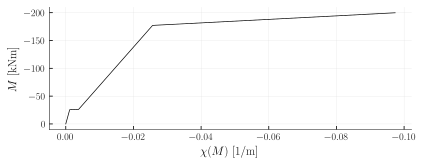
\includegraphics{index_files/mediabag/06_Versuch_2_A3_Jaeger_files/figure-pdf/fig-mchi_diagramm-output-1.pdf}

}

\caption{\label{fig-mchi_diagramm}Momenten-Krümmungsdiagramm händisch
ermittelt, definiert im positiven Bereich}

\end{figure}

\hypertarget{zustandslinien-der-kruxfcmmung}{%
\subsubsection{Zustandslinien der
Krümmung}\label{zustandslinien-der-kruxfcmmung}}

Der Biegemomentenverlauf \(M(x)\) als Eingabe in die Funktion der
Krümmung \(\chi(M)\) resultiert zu den Zustandslinie der Krümmung in
Abbildung~\ref{fig-chi_x_diagramm}. Dargestellt sind die
Krümmungsverläufe für die Biegemomentenverläufe aus
Abbildung~\ref{fig-m_x} und Abbildung~\ref{fig-m_x_versatz}.

\begin{figure}[H]

{\centering 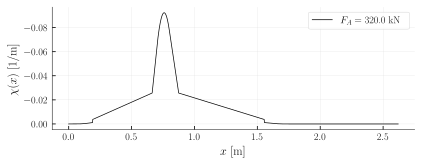
\includegraphics{index_files/mediabag/06_Versuch_2_A3_Jaeger_files/figure-pdf/fig-chi_x_diagramm-output-1.pdf}

}

\caption{\label{fig-chi_x_diagramm}Krümmungsverlauf entlang der
Stabachse}

\end{figure}

\hypertarget{punktuelle-bestimmung-der-verformung}{%
\subsubsection{Punktuelle Bestimmung der
Verformung}\label{punktuelle-bestimmung-der-verformung}}

Unter Anwendung der Arbeitsgleichung kann die Verformung nach
Gleichung~\ref{eq-arbeitsgleichung} bestimmt werden.

\begin{equation}\protect\hypertarget{eq-arbeitsgleichung}{}{
w = \int_0^l \bar{M}(x) \cdot \frac{M(x)}{EI} d_x
}\label{eq-arbeitsgleichung}\end{equation}

Wobei \(\frac{M(x)}{EI} = \chi(x)\) gilt.

Es gilt die Zustandslinien der Krümmung multipliziert mit der
Zustandslinie der Biegemomente in
Abbildung~\ref{fig-m_x_diagramm_virtuell} des virtuellen Kräftezustands
über die Stablänge zu integrieren.

\begin{figure}[H]

{\centering 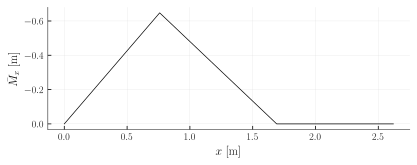
\includegraphics{index_files/mediabag/06_Versuch_2_A3_Jaeger_files/figure-pdf/fig-m_x_diagramm_virtuell-output-1.pdf}

}

\caption{\label{fig-m_x_diagramm_virtuell}Biegemomentenverlauf für den
virtuellen Kräftezustand}

\end{figure}

Für die maximale Last beträgt die Deformation an der Stelle \(w_1\)
beispielsweise:

\begin{equation}w_{1} = 14.7 \text{mm}\end{equation}

\hypertarget{zugversteifung}{%
\subsection{Zugversteifung}\label{zugversteifung}}

Die bisherige Betrachtung beschränkt sich auf einen schlagartigen
Wechsel von ungerissen zu vollständig gerissen. Dabei wird der Bereich
zwischen den Rissen ebenfalls als gerissen angenommen. Mittels der
Zugversteifung wird ein theoretischer Rissabstand ermittelt und zwischen
den Rissen eine versteifte Wirkung zwischen Betonstahl und Beton
angenommen (Verbundwirkung). Dies wird folgend auf das Versuchsbeispiel
angewendet. Berücksichtigt wird dies unter dem Ansatz von Marti,
beschrieben in Spathelf (\protect\hyperlink{ref-Spathelf2022}{2022}).

Die Krümmungsdifferenez nach Marti beträgt:

\begin{equation}\Delta\chi{\left(\lambda \right)} = \frac{\lambda}{2} \frac{f_{ct} \left(1 - \rho_{eff}\right)}{E_{s} \rho_{eff} \left(d - x_{2}\right)}\end{equation}

Der mechanische Bewehrungsgehalt folgt zu:

\begin{equation}\rho_{eff} = \frac{1}{- n + 1 + \frac{E_{s} M_{r} \left(d - x_{2}\right)}{EI^{II} f_{ct}}}\end{equation}

Eine Abschätzung des Rissabstands ist der folgende:

\begin{equation}s_{rm} = \frac{\oslash_{s} \lambda \left(1 - \rho_{eff}\right)}{4 \rho_{eff}}\end{equation}

Die Rissspannung beträgt:

\begin{equation}\sigma_{sr0} = \frac{F_{z,2}}{A_{s}}\end{equation}

und die Rissbreiten lässt sich folgend beschreiben:

\begin{equation}w_{r} = \frac{s_{rm} \left(- \lambda \sigma_{sr0} + 2 \sigma_{sr}\right)}{2 E_{s}}\end{equation}

Durch das Einsetzen der Versuchsparameter ergeben sich folgende Werte:

\begin{equation}\Delta\chi{\left(\lambda \right)} = \frac{0.00131 \lambda}{\text{m}}\end{equation}

\begin{equation}\rho_{eff} = 0.0753\end{equation}

\begin{equation}s_{rm} = 36.8 \lambda \text{mm}\end{equation}

Unter Berücksichtigung der beiden \(\lambda\)-Grenzwerte ist der
Einfluss der Zugversteifung im Momente-Krümmungsdiagramm in
Abbildung~\ref{fig-mchi_diagramm_zugversteifung} gezeigt.

\begin{figure}[H]

{\centering 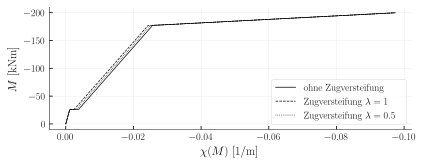
\includegraphics{index_files/mediabag/06_Versuch_2_A3_Jaeger_files/figure-pdf/fig-mchi_diagramm_zugversteifung-output-1.pdf}

}

\caption{\label{fig-mchi_diagramm_zugversteifung}Momenten-Krümmungsdiagramm
mit Zugversteifung ergänzt}

\end{figure}

Es zeigt sich ein steiferes Verhalten im ungerissenen Bereich.

\hypertarget{fachwerk}{%
\section{Fachwerk}\label{fachwerk}}

Die bisherigen Analysen beschränken sich auf eine
Querschnittsbetrachtung. Der Kraftfluss lässt sich mit einem
Spannungsfeld detaillierter verfolgen. Eine Einteilung in Parallelfelder
und Fächer ist in Abbildung~\ref{fig-spannungsfelder_steil} gezeigt.
Dabei ist der Neigungswinkel maximal steil gewählt. Die Höhe der
Spannungsfelder entspricht dem Hebelarm der inneren Kräfte.
Grundsätzlich ist dieser abhängig von der Druckzonenhöhe und der
statischen Höhe. Dies zeigte sich bereits bei der Querschnittsanalyse
zwischen den Zuständen 1 bis 4. Als Vereinfachung wird eine konstante
Höhe vorausgesetzt.

\begin{figure}[H]

{\centering 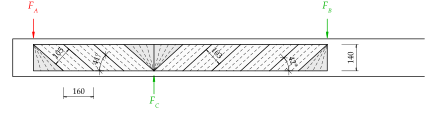
\includegraphics{index_files/mediabag/../images/Spannungsfelder.pdf}

}

\caption{\label{fig-spannungsfelder_steil}Spannungsfeld mit steiler
Feldneigung}

\end{figure}

Durch das Zusammenfassen der Felder zu Streben resultiert das Fachwerk
in Abbildung~\ref{fig-fachwerk}. Um aus dem Fachwerkmodell zutreffende
Deformation zu ermitteln, gilt es den Pendelstäben passende
Dehnsteifigkeiten zu zuordnen.

\begin{figure}[H]

{\centering 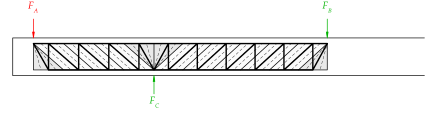
\includegraphics{index_files/mediabag/../images/Fachwerk.pdf}

}

\caption{\label{fig-fachwerk}Fachwerk mit steiler Feldneigung}

\end{figure}

\textbf{Zuggurt:}

Die Steifigkeit des Zuggurts resultiert aus der Querschnittsfläche der
Biegebewehrung und dem Elastizitätsmodul. Dabei wird die
Spannungs-Dehnungs-Beziehung gemäss Abbildung~\ref{fig-stahlkennlinie}
hinterlegt.

\textbf{Druckgurt:}

Die Querschnittsfläche des Druckgurts entspricht der Druckzonenhöhe
multipliziert mit der Plattenstreifenbreite. Diese wird als konstant
über sämtliche Stäbe des Druckgurtes angenommen. Der Elastizitätsmodul
folgt aus der Kennlinie in Abbildung~\ref{fig-betonkennlinie}.

\textbf{Druckdiagonalen:}

Die Breite der Druckdiagonalen entspricht der Breite des Spannungsfelds.
Vereinfacht gilt dies auch für die Fächer. Die Breite Multipliziert mit
der Plattenbreite resultiert zur Querschnittsfläche. Der
Elastizitätsmodul folgt ebenfalls aus
Abbildung~\ref{fig-betonkennlinie}.

\textbf{Zugstreben:}

Die vertikalen Zugstreben bilden die Schubbewehrung ab. Die
Querschnittsfläche resultiert aus der Anzahl an Schubdübeln im
entsprechenden Spannungsfeld.

\begin{figure}[H]

{\centering 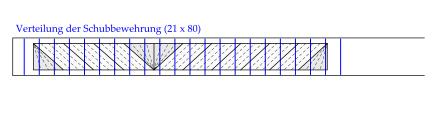
\includegraphics{index_files/mediabag/../images/Schubbewehrung_aufteilung.pdf}

}

\caption{\label{fig-schubbew_fw_steil}Anordnung der Schubbewehrung im
Fachwerk mit steiler Neigung}

\end{figure}

Das Spannungsfeld für die gewählte Neigung umfasst zwei Stabreihen. Es
ist ein linear elastisches Stoffgesetz hinterlegt.

Die Berechnung der Spannungen des Systems in @☻fig-fachwerk mit den
entsprechenden Steifigkeiten führt bei der maximalen Laststufe zu einem
Versagen der Schubbewehrung. Dies entspricht nicht dem Versagen im
Versuchsbericht. Ein angepasstes Modell ist in
Abbildung~\ref{fig-spannungsfelder_flach} gezeigt. Durch eine flachere
Neigung der Felder lagert sich die Kraft der Schubbewehrung in die
Gurtkräfte um. Die Spannungen in den Schubdübeln reduzieren sich.

\begin{figure}[H]

{\centering 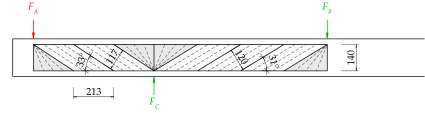
\includegraphics{index_files/mediabag/../images/Spannungsfelder_flach.pdf}

}

\caption{\label{fig-spannungsfelder_flach}Spannungsfeld mit flacher
Feldneigung}

\end{figure}

Die Querschnittsflächen der Druckdiagonalen und Zugstreben in
Abbildung~\ref{fig-fachwerk_flach} ändern sich im Vergleich mit deren
aus Abbildung~\ref{fig-fachwerk}.

\begin{figure}[H]

{\centering 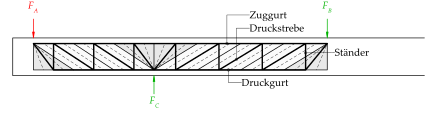
\includegraphics{index_files/mediabag/../images/Fachwerk_flach.pdf}

}

\caption{\label{fig-fachwerk_flach}Fachwerk mit flacher Feldneigung}

\end{figure}

Abbildung~\ref{fig-schubbew_fw_flach} zeigt die Erhöhung der
Querschnittsfläche der Schubbewehrung pro Strebe durch die Änderung der
Feldneigung.

\begin{figure}[H]

{\centering 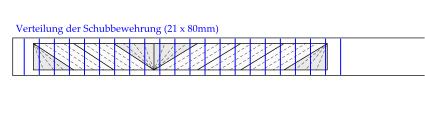
\includegraphics{index_files/mediabag/../images/Schubbewehrung_aufteilung_flach.pdf}

}

\caption{\label{fig-schubbew_fw_flach}Anordnung der Schubbewehrung im
Fachwerk mit flacher Neigung}

\end{figure}

Die Reduktion des Neigungswinkels führt zu einem Versagen der
Zugbewehrung. Das erhoffte Versagen in der Druckzone tritt nicht ein.
Dazu sind die berechneten Verformungen deutlich grösser als die
gemessenen im Versuch.

Am Fachwerkmodell lassen sich die Verformungsanteile aus der
Schubbewehrung, der Gurte und der Betondruckstreben ermitteln.
Beispielsweise lässt sich der Anteil der Schubbewehrung durch das Setzen
der Steifigkeit der übrigen Stäbe auf ein infinit grosses Mass
bestimmen. Dargestellt ist dies in
Abbildung~\ref{fig-last_verformung_fachwerk}.

\newpage{}

\hypertarget{modellvergleich}{%
\section{Modellvergleich}\label{modellvergleich}}

Abgeschlossen wird die Analyse des Dreipunktbiegeversuchs mit einer
Gegenüberstellung der angewendeten Methoden.

Der Vergleich im Momentenkrümmungsdiagramm
Abbildung~\ref{fig-mchi_diagramm_vergleich} ist Belastungsunabhängig. Es
zeigt den minimalen Einfluss der Zugversteifung.

\begin{figure}[H]

{\centering 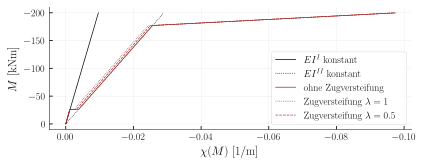
\includegraphics{index_files/mediabag/06_Versuch_2_A3_Jaeger_files/figure-pdf/fig-mchi_diagramm_vergleich-output-1.pdf}

}

\caption{\label{fig-mchi_diagramm_vergleich}Momenten-Krümmungsdiagramm
der unterschiedlichen Methoden}

\end{figure}

Der Krümmungsverlauf bedingt einen Biegemomentenverlauf. Unterschieden
wird zwischen der Berücksichtigung der Längszugkraft aus Querkraft,
siehe Abbildung~\ref{fig-chi_x_diagramm_vergleich} und
Abbildung~\ref{fig-chi_x_diagramm_laengszugkraft}.

\begin{figure}[H]

{\centering 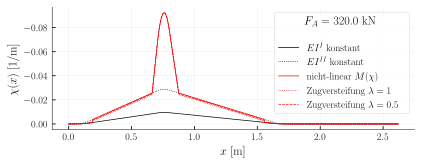
\includegraphics{index_files/mediabag/06_Versuch_2_A3_Jaeger_files/figure-pdf/fig-chi_x_diagramm_vergleich-output-1.pdf}

}

\caption{\label{fig-chi_x_diagramm_vergleich}Krümmungsverlauf für die
maximale Laststufe ohne Längszugkraft}

\end{figure}

\begin{figure}[H]

{\centering 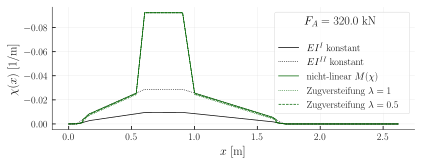
\includegraphics{index_files/mediabag/06_Versuch_2_A3_Jaeger_files/figure-pdf/fig-chi_x_diagramm_laengszugkraft-output-1.pdf}

}

\caption{\label{fig-chi_x_diagramm_laengszugkraft}Krümmungsverlauf für
die maximale Laststufe mit Längszugkraft durch Querkraft}

\end{figure}

Der Vergleich der Krümmungsverläufe zeigt, dass mit einer konstanten
Biegesteifigkeit im Bereich des Fliessens signifikante unterschiede zum
verfeinerten Momenten-Krümmungsdiagramm entstehen.

Aussagekräfte sind vor allem die Last-Verformungsdiagramme in
Abbildung~\ref{fig-last_verformung_vergleich} und
Abbildung~\ref{fig-last_verformung_laengszug}. Diese unterscheiden sich
in der Berücksichtigung der Längszugkraft aus Querkraft.

\begin{figure}[H]

{\centering 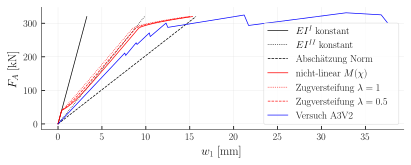
\includegraphics{index_files/mediabag/06_Versuch_2_A3_Jaeger_files/figure-pdf/fig-last_verformung_vergleich-output-1.pdf}

}

\caption{\label{fig-last_verformung_vergleich}Last-Verformungsdiagramm
bei der Krafteinleitung \(F_A\)}

\end{figure}

Es zeigt sich, dass mit einer konstanten ungerissenen Biegesteifigkeit
die Verformungen nicht zufriedenstellen abbildbar sind. Vor allem im
Bereich des Fliessens ist das Modell grundsätzlich nicht mehr
zielführend anwendbar.

Mit einer konstanten gerissenen Biegesteifigkeit nähert man sich den
Versuchsergebnissen an. Auch hier ist klar der Bereich des Fliessens des
Betonstahls nicht abgedeckt. Für eine Bemessung ist dies jedoch
zutreffend, da die Bauteile grundsätzlich nicht bis in den Fliessbereich
zu belasten sind.

Die Darstellung der Normabschätzung zeigt eine konservative Abschätzung
der Verformungen. Dies führt grundsätzlich zu einer Überbemessung. Die
Anwendung des Berechnungsalgorithmus ist jedoch simpel und somit eine
solide Grundabschätzung.

Bei der Berücksichtigung des verfeinerten Momenten-Krümmungsdiagramms in
rot dargestellt, lässt sich das Verformungsverhalten des Versuchs
annähernd abbilden. Das Modell bildet ein zu steifes Verhalten ab. Die
Zugversteifung wirkt der Modellgenauigkeit entgegen.

\begin{figure}[H]

{\centering 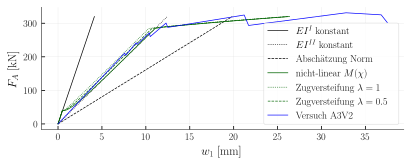
\includegraphics{index_files/mediabag/06_Versuch_2_A3_Jaeger_files/figure-pdf/fig-last_verformung_laengszug-output-1.pdf}

}

\caption{\label{fig-last_verformung_laengszug}Last-Verformungsdiagramm
bei der Krafteinleitung \(F_A\) mit Längszugkraft aus Querkraft}

\end{figure}

Die Abbildung~\ref{fig-last_verformung_laengszug} zeigt sämtliche
Berechnungsmethoden unter Berücksichtung der Längszugkraft aus
Querkraft. Es zeigt sich deutlich, dass das Berechnungsmodell mit der
Zugversteifung den Versuchsverlauf zufriedenstellend abbildet. Lediglich
Abweichungen im höchstlastbereich sind vorhanden.

Die Normabschätzung zeigt deutliche Abweichungen zu den gemessenen
Verformungen. Zwar liegen diese auf der sicheren Seite, sind jedoch
äusserst konservativ.

\begin{figure}[H]

{\centering 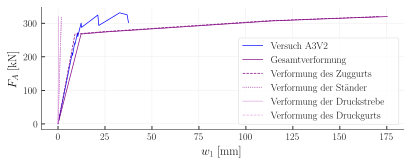
\includegraphics{index_files/mediabag/06_Versuch_2_A3_Jaeger_files/figure-pdf/fig-last_verformung_fachwerk-output-1.pdf}

}

\caption{\label{fig-last_verformung_fachwerk}Last-Verformungsdiagramm
bei der Krafteinleitung \(F_A\) mittels Fachwerkmodell}

\end{figure}

Das Fachwerkmodell beschreibt den Verlauf ausreichend präzise. Die
maximale Deformation mit der rechnerisch ermittelten Höhe, sprich
innerem Hebelarm aus der Querschnittsnalyse überschiesst das Ziel bei
Weitem. Das Fachwerkmodell reagiert äusserst sensitiv auf die gewählte
Höhe. Der Verformungsverlauf lässt sich mit einer Fachwerkshöhe von
\(160mm\) präzise abbilden. Ohne Kenntnisse der Versuchsresultate wäre
jedoch eine präzise Bestimmung der Verformung im Bereich des Fliessens
der Zugbewehrung nicht möglich.

\bookmarksetup{startatroot}

\hypertarget{numerische-integration-der-kruxfcmmung-2}{%
\chapter{Numerische Integration der
Krümmung}\label{numerische-integration-der-kruxfcmmung-2}}

\hypertarget{grundlagen-1}{%
\subsection{Grundlagen}\label{grundlagen-1}}

Um sich von der Betrachtung einer konstanten Biegesteifigkeit zu lösen,
hilft die Anwendung einer verfeinerten Momenten-Krümmungsbeziehung.
Folgend wird ein Momentenkrümmungsdiagramm für den Querschnitt aus dem
beschriebenen Versuch berechnet. Die vorhandene Querkraftbewehrung ist
nicht dargestellt in Abbildung~\ref{fig-qs_a3}.

\begin{figure}[H]

{\centering 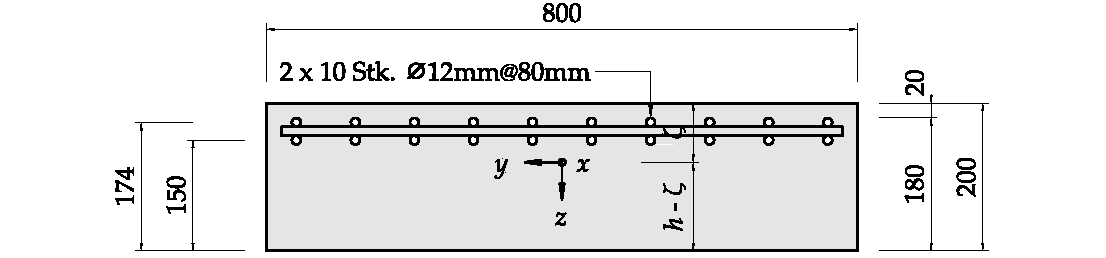
\includegraphics{index_files/mediabag/../images/QS_Versuch_A3.pdf}

}

\caption{\label{fig-qs_a3}Querschnitt des Versuchs A3 zur Bestimmung des
Momenten-Krümmungdiagramms}

\end{figure}

Vereinfacht wird der Querschnitt folgender massen:

\begin{figure}[H]

{\centering 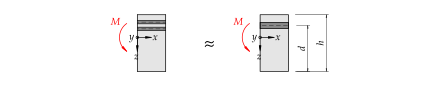
\includegraphics{index_files/mediabag/../images/QS_analyse_1.pdf}

}

\caption{Vereinfachung der Bewehrungsführung}

\end{figure}

Die Parameter in Tabelle~\ref{tbl-params_krummung} finden Einfluss in
die Berechnungen.

\hypertarget{tbl-params_krummung}{}
\begin{longtable}[]{@{}
  >{\raggedright\arraybackslash}p{(\columnwidth - 2\tabcolsep) * \real{0.5000}}
  >{\raggedright\arraybackslash}p{(\columnwidth - 2\tabcolsep) * \real{0.5000}}@{}}
\caption{\label{tbl-params_krummung}Versuchsparameter für die
verfeinerte Momenten-Krümmungsbeziehung}\tabularnewline
\toprule\noalign{}
\endfirsthead
\endhead
\bottomrule\noalign{}
\endlastfoot
\(E_{c} = 30000.0 \, \frac{\text{N}}{\text{mm}^{2}}\) &
\(E_{s} = 200000.0 \, \frac{\text{N}}{\text{mm}^{2}}\) \\
\(\oslash_{s} = 18.0 \, \text{mm}\) & \(c_{nom} = 20.0 \, \text{mm}\) \\
\(f_{c} = 35.0 \, \frac{\text{N}}{\text{mm}^{2}}\) &
\(f_{ct} = 4.0 \, \frac{\text{N}}{\text{mm}^{2}}\) \\
\(f_{s550} = 550.0 \, \frac{\text{N}}{\text{mm}^{2}}\) &
\(f_{su} = 800 \, \frac{\text{N}}{\text{mm}^{2}}\) \\
\(f_{sy} = 670.0 \, \frac{\text{N}}{\text{mm}^{2}}\) &
\(\varepsilon_{cu} = 0.003\) \\
\(\varepsilon_{su} = 0.5\) & \\
\end{longtable}

Neben den Parametern wird das Stoffgesetz für den Betonstahl in
Abbildung~\ref{fig-stahlkennlinie} hinterlegt. Das Bilineare, bzw.
linear-elastisch linear-plastische Spannungs-Dehnungsdiagramm für den
Betonstahl hält den Rechenaufwand klein und liefert eine ausreichende
Genauigkeit. Eine Berücksichtigung des verfestigenden Verhaltens ist
essentiell um die Verformungen nach dem Fliessen des Betonstahls
näherungsweise zu bestimmen. Das Diagramm ist definiert bis zur
Bruchdehnung des Stahls. Das Verhalten gilt ebenso im negativen
Spannungs-Dehnungs Bereich.

\begin{figure}[H]

{\centering \includegraphics{index_files/mediabag/07_Versuch_SV14b_files/figure-pdf/fig-stahlkennlinie-output-1.pdf}

}

\caption{\label{fig-stahlkennlinie}Spannungs-Dehnungs Diagramm des
Bewehrungsstahls linear elastisch-linear verfestigend plastisch}

\end{figure}

Die Betonkennlinie in Abbildung~\ref{fig-betonkennlinie} zeigt ein
linear-elastisches ideal-plastisches verhalten. Im positiven Bereich
lässt sich die Betonspannung bis zur Betonzugfestigkeit erhöhen, im
negativen Spannungsbereich beginnt ein Plastifizieren beim Erreichen der
Betondruckfestigkeit. Bis zur Bruchstauchung ist dies definiert.

\begin{figure}[H]

{\centering \includegraphics{index_files/mediabag/07_Versuch_SV14b_files/figure-pdf/fig-betonkennlinie-output-1.pdf}

}

\caption{\label{fig-betonkennlinie}Spannungs-Dehnungs Diagramm des
Betons linear elastisch-ideal plastisch}

\end{figure}

\hypertarget{querschnittsanalyse-1}{%
\subsection{Querschnittsanalyse}\label{querschnittsanalyse-1}}

Mittels einer Querschnittsanalyse lassen sich die unterschiedlichen
Zustände des Momenten-Krümmungdiagramms ermitteln.

\hypertarget{schwerpunkt-des-querschnitts-1}{%
\subsubsection{Schwerpunkt des
Querschnitts}\label{schwerpunkt-des-querschnitts-1}}

Durch die Bestimmung der Wertigkeit \(n\) kann der Querschnitt als
homogener Betonquerschnitt zur Bestimmung des Schwerpunkts behandelt
werden.

\begin{equation}n = \frac{E_{s}}{E_{c}}\end{equation}

\begin{equation}n = 6.67\end{equation}

Die Querschnittsfläche der Bewehrung beträgt:

\begin{equation}A_{s} = \frac{36 \pi f_{s550} \text{mm}^{2}}{f_{sy}} + 2 \cdot \frac{1}{4} \pi \oslash_{s}^{2}\end{equation}

\begin{equation}A_{s} = 601.8 \text{mm}^{2}\end{equation}

Die Betonquerschnittsfläche:

\begin{equation}A_{c} = b h\end{equation}

\begin{equation}A_{c} = 76500.0 \text{mm}^{2}\end{equation}

Die ideelle Querschnittsfläche resultiert zu:

\begin{equation}A_{i} = A_{c} + A_{s} \left(n - 1\right)\end{equation}

\begin{equation}A_{i} = 79910.1 \text{mm}^{2}\end{equation}

Und die z-Koordinate des Schwerpunkts folgt abschliessend zu:

\begin{equation}\zeta_{c} = \frac{\frac{A_{c} h}{2} + A_{s} \left(1.5 \oslash_{s} + c_{nom}\right) \left(n - 1\right)}{A_{i}}\end{equation}

\begin{equation}\zeta_{c} = 217.0 \text{mm}\end{equation}

\hypertarget{fluxe4chentruxe4gheitsmoment-1}{%
\subsubsection{Flächenträgheitsmoment}\label{fluxe4chentruxe4gheitsmoment-1}}

Das Flächenträgheitsmoment wird ebenfalls am ideellen Querschnitt
bestimmt. Die Eigenträgheitsmomente der Kreisquerschnitte der Bewehrung
sind nicht berücksichtigt, lediglich der Steiner-Anteil fliesst in die
Berechnung ein:

\begin{equation}I^{I} = A_{s} \left(n - 1\right) \left(\frac{3 \oslash_{s}}{2} + c_{nom} - \zeta_{c}\right)^{2} + \frac{b h^{3}}{12} + b h \left(\frac{h}{2} - \zeta_{c}\right)^{2}\end{equation}

\begin{equation}I^{I} = 1.39 \cdot 10^{9} \text{mm}^{4}\end{equation}

\hypertarget{ungerissen---zustand-1-1}{%
\subsubsection{Ungerissen - Zustand 1}\label{ungerissen---zustand-1-1}}

Der Querschnitt verbleibt elastisch. Folglich kann das
Flächenträgheitsmoment mit \(E_c\) multipliziert werden und es
resultiert die ungerissene Biegesteifigkeit:

\begin{equation}EI^{I} = E_{c} I^{I}\end{equation}

\begin{equation}EI^{I} = 4.183 \cdot 10^{4} \text{kN} \text{m}^{2}\end{equation}

\hypertarget{rissmoment-1}{%
\paragraph{Rissmoment}\label{rissmoment-1}}

Durch die Ermittlung des Rissmoments kann die Krümmung vor dem Reissen
des Betons ermittelt werden. Die Betonzugkraft wird nicht
berücksichtigt.

\begin{figure}[H]

{\centering \includegraphics{index_files/mediabag/../images/QS_analyse_2.pdf}

}

\caption{\label{fig-qs2}Querschnittsanalyse vor dem Reissen des Betons}

\end{figure}

Die Betondruckspannung beträgt:

\begin{equation}\sigma_{c inf,1} = \frac{f_{ct} \left(h - \zeta_{c}\right)}{\zeta_{c}}\end{equation}

\begin{equation}\sigma_{c inf,1} = \frac{4.28 \text{N}}{\text{mm}^{2}}\end{equation}

Der Hebelarm der inneren Kräfte folgt zu:

\begin{equation}z_{1} = - 1.5 \oslash_{s} - c_{nom} + \frac{2 h}{3} + \frac{\zeta_{c}}{3}\end{equation}

\begin{equation}z_{1} = 326.0 \text{mm}\end{equation}

Die Betondruckkraft ist definiert nach:

\begin{equation}F_{c,1} = \frac{b \sigma_{c inf,1} \left(h - \zeta_{c}\right)}{2}\end{equation}

\begin{equation}F_{c,1} = 84.6 \text{kN}\end{equation}

Und das Rissmoment resultiert schliesslich zu:

\begin{equation}M_{r} = F_{c,1} z_{1}\end{equation}

\begin{equation}M_{r} = 27.54 \text{kN} \text{m}\end{equation}

Aus dem Rissmoment folgt die Krümmung beim Reissen:

\begin{equation}\chi_{r} = \frac{M_{r}}{EI^{I}}\end{equation}

\begin{equation}\chi_{r} = \frac{0.000659}{\text{m}}\end{equation}

Die Neigung linearen Funktion des ungerissenen Zustands im
Momentenkrümmungsdiagramm ist durch die Biegesteifigkeit definiert. Der
Endpunkts des Zustand 1 definiert das Rissmoment mit der entsprechenden
Krümmung.

\hypertarget{gerissen-elastisch---zustand-2-1}{%
\subsubsection{Gerissen Elastisch - Zustand
2}\label{gerissen-elastisch---zustand-2-1}}

Der Querschnitt nach dem Reissen ist in Abbildung~\ref{fig-qs3}
dargestellt. Der Betonstahl hat die Fliessgrenze noch nicht erreicht.
Der Beton die Druckfestigkeit ebenfalls nicht.

\begin{figure}[H]

{\centering \includegraphics{index_files/mediabag/../images/QS_analyse_3.pdf}

}

\caption{\label{fig-qs3}Querschnittsanalyse nach dem Reissen des Betons}

\end{figure}

Dabei beträgt die statische Höhe:

\begin{equation}d = - \frac{3 \oslash_{s}}{2} - c_{nom} + h\end{equation}

\begin{equation}d = 403.0 \text{mm}\end{equation}

Mittels Gleichgewicht der Kräfte lässt sich die Betondruckzonenhöhe und
folglich die gerissene Biegesteifigkeit herleiten. Die
Betonstahlzugkraft beträgt:

\begin{equation}F_{z,2} = A_{s} \sigma_{s,2}\end{equation}

Die Betonstahlspannung für linear elastisches Verhalten folgt zu:

\begin{equation}\sigma_{s,2} = E_{s} \varepsilon_{s,2}\end{equation}

Die Betondruckkraft anhand des dreieckigen Verlaufs in
Abbildung~\ref{fig-qs3} beträgt:

\begin{equation}F_{c,2} = \frac{b \sigma_{c inf,2} x_{2}}{2}\end{equation}

Die Betonspannung ebenfalls bestimmt durch ein linear elastisches
Verhalten ist definiert durch:

\begin{equation}\sigma_{c inf,2} = E_{c} \varepsilon_{c,2}\end{equation}

Die Betondehnung anhand des Dehnungsverlaufs in Abbildung~\ref{fig-qs3}:

\begin{equation}\varepsilon_{c,2} = \frac{\varepsilon_{s,2} x_{2}}{d - x_{2}}\end{equation}

Unter Bemühung des Gleichgewichts der horizontalen Kräfte lässt sich die
folgende Beziehung ermitteln.

\begin{equation}F_{c,2} = F_{z,2}\end{equation}

Einsetzen der bestimmten Gleichungen in die Gleichgewichtsbeziehung und
mit \(n\) und \(\rho\) substituiert, folgt:

\begin{equation}n = \frac{E_{s}}{E_{c}}\end{equation}

\begin{equation}\rho = \frac{A_{s}}{b d}\end{equation}

\begin{equation}E_{s} b d \rho \varepsilon_{s,2} = \frac{E_{s} b \varepsilon_{s,2} x_{2}^{2}}{2 n \left(d - x_{2}\right)}\end{equation}

Durch die Auflösung nach \(x\) folgt die Betondruckzonenhöhe:

\begin{equation}x_{2} = d \left(- n \rho + \sqrt{n \rho \left(n \rho + 2\right)}\right)\end{equation}

\begin{equation}x_{2} = 116.0 \text{mm}\end{equation}

Zur Bestimmung der Krümmung ist die Betonstahldehnung erforderlich.
Diese bedingt ein einwirkendes Moment. Der Übergang zwischen
ungerissenem zu gerissenem Verhalten erfolgt beim Rissmoment. Folglich
kann das Rissmoment in Abbildung~\ref{fig-qs3} angesetzt werden.

\begin{equation}M_{2} = F_{z,2} \left(d - \frac{x_{2}}{3}\right)\end{equation}

\begin{equation}M_{2} = M_{r}\end{equation}

\begin{equation}M_{r} = A_{s} E_{s} \varepsilon_{s,2} \left(d - \frac{x_{2}}{3}\right)\end{equation}

Daraus resultiert die Betonstahldehnung:

\begin{equation}\varepsilon_{s,2} = 0.000628\end{equation}

Die Krümmung kann anhand des Dehnungsverlaufs in Abbildung~\ref{fig-qs3}
bestimmt werden:

\begin{equation}\chi^{II} = \frac{\varepsilon_{s,2}}{d - x_{2}}\end{equation}

\begin{equation}\chi^{II} = \frac{0.00219}{\text{m}}\end{equation}

Abschliessend folgt die gerissene Biegesteifigkeit zu:

\begin{equation}EI^{II} = \frac{M_{2}}{\chi^{II}}\end{equation}

\begin{equation}EI^{II} = 12567.0 \text{kN} \text{m}^{2}\end{equation}

Die Neigung der linearen Funktion im gerissenen Bereich ist durch die
gerissene Biegesteifigkeit definiert. Der Beginn ist durch das
Rissmoment definiert.

\hypertarget{fliessen-der-bewehrung---zustand-3-1}{%
\subsubsection{Fliessen der Bewehrung - Zustand
3}\label{fliessen-der-bewehrung---zustand-3-1}}

Die Biegesteifigkeit \(EI^{II}\) gilt bis die Bewehrung fliesst oder der
Beton beginnt zu plastifizieren. In Abbildung~\ref{fig-qs4} wird
vorausgesetzt, dass die Bewehrung fliesst.

\begin{figure}[H]

{\centering \includegraphics{index_files/mediabag/../images/QS_analyse_4.pdf}

}

\caption{\label{fig-qs4}Querschnittsanalyse für reine Biegung beim
Fliessen der Bewehrung}

\end{figure}

Durch Gleichgewicht der horizontalen Kräfte folgen die Beziehungen:

\begin{equation}\sigma_{c inf,3} = \frac{E_{c} f_{sy} x_{3}}{E_{s} \left(d - x_{3}\right)}\end{equation}

\begin{equation}A_{s} f_{sy} = \frac{b \sigma_{c inf,3} x_{3}}{2}\end{equation}

Aufgelöst nach der Druckzonenhöhe:

\begin{equation}x_{3} = \frac{- A_{s} E_{s} + \sqrt{A_{s} E_{s} \left(A_{s} E_{s} + 2 E_{c} b d\right)}}{E_{c} b}\end{equation}

\begin{equation}x_{3} = 116.0 \text{mm}\end{equation}

Daraus lässt sich das Fliessmoment bestimmen, welches den Endpunkt im
Momenten-Krümmungsdiagramm für den gerissenen Zustand definiert:

\begin{equation}M_{y} = A_{s} f_{sy} \left(d - \frac{x_{3}}{3}\right)\end{equation}

\begin{equation}M_{y} = 146.9 \text{kN} \text{m}\end{equation}

Die Fliessdehnung des Betonstahls entspricht:

\begin{equation}\varepsilon_{sy} = 0.00335\end{equation}

Abschliessend lässt sich die Krümmung für den Endpunkt des Zustands 2
folgend bestimmen:

\begin{equation}\chi_{y} = \frac{\varepsilon_{sy}}{d - x_{3}}\end{equation}

\begin{equation}\chi_{y} = \frac{0.0117}{\text{m}}\end{equation}

Der Zustand 3 beschreibt lediglich den Endpunkt des gerissenen Bereichs
im Momenten-Krümmungsdiagramm.

\hypertarget{maximaler-biegewiderstand---zustand-4-1}{%
\subsubsection{Maximaler Biegewiderstand - Zustand
4}\label{maximaler-biegewiderstand---zustand-4-1}}

Abschliessen kann der maximale Biegewiderstand durch die plastifizierung
der Betondruckzone bestimmt werden. Vereinfacht wird dem Betonstahl die
statische Zugfestigkeit vorausgesetzt um das verfestigende Verhalten
annähernd abzubilden. Dies bedingt grundsätzlich das Erreichen der
Bruchdehnung im Stahl. Da der Querschnitt stark bewehrt ist, versagt die
Betondruckzone vor dem Erreichen der Betonstahlbruchdehnung.

\begin{figure}[H]

{\centering \includegraphics{index_files/mediabag/../images/QS_analyse_5.pdf}

}

\caption{\label{fig-qs5}Querschnittsanalyse für reine Biegung mit der
Bewehrung bei der Bruchspannung und plastifizierter Betondruckzone}

\end{figure}

Vereinfacht werden die Spannungen in der Druckzone konstant verteilt
betrachtet. Dazu wird die Druckzonenhöhe abgemindert um Faktor 0.85.

Das Gleichgewicht der Kräfte führt zu:

\begin{equation}A_{s} f_{su} = 0.85 b f_{c} x_{4}\end{equation}

Die Druckzonenhöhe folgt zu:

\begin{equation}x_{4} = 95.2 \text{mm}\end{equation}

Der maximale Biegewiderstand folgt zu:

\begin{equation}M_{R} = A_{s} f_{su} \left(d - 0.425 x_{4}\right)\end{equation}

\begin{equation}M_{R} = 174.5 \text{kN} \text{m}\end{equation}

Die Krümmung lässt sich anhand der Betonstauchung ermitteln:

\begin{equation}\chi_{u} = \frac{\varepsilon_{cu}}{x_{4}}\end{equation}

\begin{equation}\chi_{u} = \frac{0.0315}{\text{m}}\end{equation}

Die Betonstahldehnung darf die Bruchdehnung nicht überschreiten:

\begin{equation}\varepsilon_{s,4} = \frac{\varepsilon_{cu} \left(d - x_{4}\right)}{x_{4}}\end{equation}

\begin{equation}\varepsilon_{s,4} = 0.0097\end{equation}

Die Bruchdehnung des Stahls wird nicht erreicht. Der Querschnitt versagt
im Druckbereich. Die Annahme, dem Betonstahl die statische Zugfestigkeit
zu Grunde zu legen ist grundsätzlich nicht gerechtfertig. Der Vergleich
mit den Versuchsergebnissen zeigt jedoch, dass sich diese Annahme
bewährt.

\begin{equation}\varepsilon_{su} = 0.5\end{equation}

Die Biegesteifigkeit im Bereich 3 beträgt:

\begin{equation}EI^{III} = \frac{M_{R}}{\chi_{u}}\end{equation}

\begin{equation}EI^{III} = 5.54 \cdot 10^{3} \text{kN} \text{m}^{2}\end{equation}

Der Zustand 4 beschreibt den Endpunkt des Momenten-Krümmungsdiagramm.

\hypertarget{momenten-kruxfcmmungsdiagramm-2}{%
\subsubsection{Momenten-Krümmungsdiagramm}\label{momenten-kruxfcmmungsdiagramm-2}}

Abschliessend lässt sich aus der Querschnittsanalyse die Beziehung
zwischen Biegemoment und Krümmung ermitteln. Der lineare verlauf im
ersten Bereich ergibt sich aus der ungerissenen Biegesteifigkeit. Darauf
folgt ein schlagartiger wechsel der Steifigkeit von \(EI^I\) zu
\(EI^{II}\), da der Beton reisst. Dies führt zum Plateau im unteren
Bereich. Im Bereich drei werden die zwei definierten Punkte
\(M_y, \chi_y\) sowie \(M_R, \chi_u\) linear verbunden.

\begin{figure}[H]

{\centering \includegraphics{index_files/mediabag/07_Versuch_SV14b_files/figure-pdf/fig-mchi_diagramm-output-1.pdf}

}

\caption{\label{fig-mchi_diagramm}Momenten-Krümmungsdiagramm händisch
ermittelt, definiert im positiven Bereich}

\end{figure}

\begin{equation}259.485759493671\end{equation}

\bookmarksetup{startatroot}

\hypertarget{verformung-an-einem-einfachen-balken}{%
\chapter{Verformung an einem einfachen
Balken}\label{verformung-an-einem-einfachen-balken}}

\hypertarget{numerische-integration-der-kruxfcmmungen}{%
\section{Numerische Integration der
Krümmungen}\label{numerische-integration-der-kruxfcmmungen}}

Zur Näherung an die Praxisanwendung ist die Momenten-Krümmungsbeziehung
mittels einer FEM-Software ermittelt worden.

\begin{equation}715.424\end{equation}

\begin{verbatim}
c:\Users\Pascal Gitz\OneDrive - Hochschule Luzern\02_Master\03_Tragverhalten_von_Stahlbetontragwerken\docs
\end{verbatim}

\begin{figure}[H]

{\centering \includegraphics{index_files/mediabag/07_Versuch_SV14b_files/figure-pdf/cell-62-output-1.pdf}

}

\end{figure}

$[0,~5.015015 \times 10^{-5},~0.0001003003,~\dots,~0.0499997,~0.05004985,~0.0501] \; \mathrm{\frac{1}{m}}$

\begin{figure}[H]

{\centering \includegraphics{index_files/mediabag/07_Versuch_SV14b_files/figure-pdf/cell-65-output-1.pdf}

}

\end{figure}

\begin{verbatim}
array([0.00000000e+00, 7.32936326e-03, 1.46587265e-02, 2.19880898e-02,
       2.93174530e-02, 3.66468163e-02, 4.39761796e-02, 5.13089535e-02,
       5.86599527e-02, 6.60109519e-02, 7.33619511e-02, 8.07129503e-02,
       8.80639495e-02, 9.54149487e-02, 1.05135135e-01, 1.19549550e-01,
       1.33963964e-01, 1.48378378e-01, 1.62792793e-01, 1.77207207e-01,
       1.91621622e-01, 2.06036036e-01, 2.20450450e-01, 2.34864865e-01,
       2.49279279e-01, 2.63563267e-01, 2.77832426e-01, 2.92101586e-01,
       3.04427832e-01, 3.13628522e-01, 3.22829212e-01, 3.32029902e-01,
       3.41230592e-01, 3.50431282e-01, 3.56712281e-01, 3.62782401e-01,
       3.68852521e-01, 3.74922641e-01, 3.80992760e-01, 3.87062880e-01,
       3.93133000e-01, 3.99203120e-01, 4.06036036e-01, 4.13243243e-01,
       4.20450450e-01, 4.27657658e-01, 4.34864865e-01, 4.42072072e-01,
       4.49279279e-01, 4.56565849e-01, 4.63884442e-01, 4.71203035e-01,
       4.78521628e-01, 4.85840221e-01, 4.93158814e-01, 5.00477407e-01,
       5.14109024e-01, 5.28767751e-01, 5.43426477e-01, 5.58085204e-01,
       5.72743930e-01, 5.87402657e-01, 6.02061383e-01, 6.16720110e-01,
       6.31378836e-01, 6.46037563e-01, 6.60820197e-01, 6.75686638e-01,
       6.90553080e-01, 7.07008704e-01, 7.28996793e-01, 7.50984883e-01,
       7.72972973e-01, 7.94961063e-01, 8.16949153e-01, 8.38937242e-01,
       8.60925332e-01, 8.82913422e-01, 9.04901512e-01, 9.26889601e-01,
       9.48877691e-01, 9.70847518e-01, 9.92813314e-01, 1.01459459e+00,
       1.03621622e+00, 1.05783784e+00, 1.07945946e+00, 1.10108108e+00,
       1.12270270e+00, 1.14432432e+00, 1.16594595e+00, 1.18756757e+00,
       1.20918919e+00, 1.23081081e+00, 1.25243243e+00, 1.27447753e+00,
       1.29655018e+00, 1.32345396e+00, 1.35277142e+00, 1.38208887e+00,
       1.41140632e+00, 1.44072377e+00, 1.47004123e+00, 1.49935868e+00,
       1.52867613e+00, 1.55799359e+00, 1.58731104e+00, 1.61662849e+00,
       1.64594595e+00, 1.67522842e+00, 1.70449538e+00, 1.73333333e+00,
       1.76216216e+00, 1.79099099e+00, 1.81981982e+00, 1.84864865e+00,
       1.87747748e+00, 1.90630631e+00, 1.93513514e+00, 1.96396396e+00,
       1.99279279e+00, 2.02162162e+00, 2.05045045e+00, 2.07932784e+00,
       2.10824553e+00, 2.13756299e+00, 2.16688044e+00, 2.19619789e+00,
       2.22551535e+00, 2.25483280e+00, 2.28415025e+00, 2.31346770e+00,
       2.34278516e+00, 2.37210261e+00, 2.40142006e+00, 2.43073752e+00,
       2.46004814e+00, 2.48929140e+00, 2.51837838e+00, 2.54720721e+00,
       2.57603604e+00, 2.60486486e+00, 2.63369369e+00, 2.66252252e+00,
       2.69135135e+00, 2.72018018e+00, 2.74900901e+00, 2.77783784e+00,
       2.80666667e+00, 2.83549550e+00, 2.86454614e+00, 2.89448405e+00,
       2.92794320e+00, 2.96459001e+00, 3.00123683e+00, 3.03788365e+00,
       3.07453046e+00, 3.11117728e+00, 3.14782410e+00, 3.18447091e+00,
       3.22111773e+00, 3.25776454e+00, 3.29441136e+00, 3.33105818e+00,
       3.36733473e+00, 3.40220662e+00, 3.43279890e+00, 3.46211635e+00,
       3.49143381e+00, 3.52075126e+00, 3.55006871e+00, 3.57938617e+00,
       3.60870362e+00, 3.63802107e+00, 3.66733852e+00, 3.69665598e+00,
       3.72597343e+00, 3.75529088e+00, 3.78451864e+00, 3.81369369e+00,
       3.84252252e+00, 3.87135135e+00, 3.90018018e+00, 3.92900901e+00,
       3.95783784e+00, 3.98666667e+00, 4.01549550e+00, 4.04432432e+00,
       4.07315315e+00, 4.10198198e+00, 4.13081081e+00, 4.15963964e+00,
       4.18994287e+00, 4.22198809e+00, 4.25863491e+00, 4.29528172e+00,
       4.33192854e+00, 4.36857536e+00, 4.40522217e+00, 4.44186899e+00,
       4.47851580e+00, 4.51516262e+00, 4.55180944e+00, 4.58845625e+00,
       4.62510307e+00, 4.66174989e+00, 4.69595508e+00, 4.72756757e+00,
       4.75639640e+00, 4.78522523e+00, 4.81405405e+00, 4.84288288e+00,
       4.87171171e+00, 4.90054054e+00, 4.92936937e+00, 4.95819820e+00,
       4.98702703e+00, 5.01585586e+00, 5.04468468e+00, 5.07355622e+00,
       5.10253254e+00, 5.13169950e+00, 5.16101695e+00, 5.19033440e+00,
       5.21965186e+00, 5.24896931e+00, 5.27828676e+00, 5.30760421e+00,
       5.33692167e+00, 5.36623912e+00, 5.39555657e+00, 5.42487403e+00,
       5.45419148e+00, 5.48471770e+00, 5.51610241e+00, 5.55267980e+00,
       5.58932661e+00, 5.62597343e+00, 5.66262025e+00, 5.69926706e+00,
       5.73591388e+00, 5.77256070e+00, 5.80920751e+00, 5.84585433e+00,
       5.88250115e+00, 5.91914796e+00, 5.95579478e+00, 5.99025989e+00,
       6.02288288e+00, 6.05171171e+00, 6.08054054e+00, 6.10936937e+00,
       6.13819820e+00, 6.16702703e+00, 6.19585586e+00, 6.22468468e+00,
       6.25351351e+00, 6.28234234e+00, 6.31117117e+00, 6.34000000e+00,
       6.36882883e+00, 6.40020306e+00, 6.43366926e+00, 6.47031608e+00,
       6.50696290e+00, 6.54360971e+00, 6.58025653e+00, 6.61690334e+00,
       6.65355016e+00, 6.69019698e+00, 6.72684379e+00, 6.76349061e+00,
       6.80013743e+00, 6.83678424e+00, 6.87314284e+00, 6.90609722e+00,
       6.93675676e+00, 6.96558559e+00, 6.99441441e+00, 7.02324324e+00,
       7.05207207e+00, 7.08090090e+00, 7.10972973e+00, 7.13855856e+00,
       7.16738739e+00, 7.19621622e+00, 7.22504505e+00, 7.25387387e+00,
       7.28382688e+00, 7.31562059e+00, 7.35130554e+00, 7.38795236e+00,
       7.42459918e+00, 7.46124599e+00, 7.49789281e+00, 7.53453962e+00,
       7.57118644e+00, 7.60783326e+00, 7.64448007e+00, 7.68112689e+00,
       7.71777371e+00, 7.75442052e+00, 7.79106734e+00, 7.82771415e+00,
       7.86436097e+00, 7.90100779e+00, 7.93765460e+00, 7.97430142e+00,
       8.01094824e+00, 8.04759505e+00, 8.08424187e+00, 8.12088869e+00,
       8.15753550e+00, 8.19418232e+00, 8.23082913e+00, 8.26747595e+00,
       8.30653029e+00, 8.34810811e+00, 8.39135135e+00, 8.43459459e+00,
       8.47783784e+00, 8.52108108e+00, 8.56432432e+00, 8.60756757e+00,
       8.65081081e+00, 8.69405405e+00, 8.73729730e+00, 8.78054054e+00,
       8.82378378e+00, 8.86702703e+00, 8.90732101e+00, 8.94535044e+00,
       8.98199725e+00, 9.01864407e+00, 9.05529088e+00, 9.09193770e+00,
       9.12858452e+00, 9.16523133e+00, 9.20187815e+00, 9.23852497e+00,
       9.27517178e+00, 9.31181860e+00, 9.34846541e+00, 9.38577293e+00,
       9.42586187e+00, 9.46891892e+00, 9.51216216e+00, 9.55540541e+00,
       9.59864865e+00, 9.64189189e+00, 9.68513514e+00, 9.72837838e+00,
       9.77162162e+00, 9.81486486e+00, 9.85810811e+00, 9.90135135e+00,
       9.94459459e+00, 9.98791806e+00, 1.00316079e+01, 1.00755841e+01,
       1.01195602e+01, 1.01635364e+01, 1.02075126e+01, 1.02514888e+01,
       1.02954650e+01, 1.03394411e+01, 1.03834173e+01, 1.04273935e+01,
       1.04713697e+01, 1.05153459e+01, 1.05593220e+01, 1.06052151e+01,
       1.06542342e+01, 1.07046847e+01, 1.07551351e+01, 1.07866667e+01,
       1.07866667e+01, 1.07866667e+01, 1.07866667e+01, 1.07866667e+01,
       1.07866667e+01, 1.07866667e+01, 1.07866667e+01, 1.07866667e+01,
       1.07866667e+01, 1.07866667e+01, 1.07866667e+01, 1.07866667e+01,
       1.07866667e+01, 1.07866667e+01, 1.07866667e+01, 1.07866667e+01,
       1.07866667e+01, 1.07866667e+01, 1.07866667e+01, 1.07866667e+01,
       1.07866667e+01, 1.07866667e+01, 1.07866667e+01, 1.07866667e+01,
       1.07866667e+01, 1.07866667e+01, 1.07866667e+01, 1.07866667e+01,
       1.07866667e+01, 1.07866667e+01, 1.07866667e+01, 1.07866667e+01,
       1.07866667e+01, 1.07866667e+01, 1.07866667e+01, 1.07866667e+01,
       1.07866667e+01, 1.07866667e+01, 1.07866667e+01, 1.07866667e+01,
       1.07866667e+01, 1.07866667e+01, 1.07866667e+01, 1.07866667e+01,
       1.07866667e+01, 1.07866667e+01, 1.07866667e+01, 1.07866667e+01,
       1.07866667e+01, 1.07866667e+01, 1.07866667e+01, 1.07866667e+01,
       1.07866667e+01, 1.07866667e+01, 1.07866667e+01, 1.07866667e+01,
       1.07866667e+01, 1.07866667e+01, 1.07866667e+01, 1.07866667e+01,
       1.07866667e+01, 1.07866667e+01, 1.07866667e+01, 1.07866667e+01,
       1.07866667e+01, 1.07866667e+01, 1.07866667e+01, 1.07866667e+01,
       1.07866667e+01, 1.07866667e+01, 1.07866667e+01, 1.07866667e+01,
       1.07866667e+01, 1.07866667e+01, 1.07866667e+01, 1.07866667e+01,
       1.07866667e+01, 1.07866667e+01, 1.07866667e+01, 1.07866667e+01,
       1.07866667e+01, 1.07866667e+01, 1.07866667e+01, 1.07866667e+01,
       1.07866667e+01, 1.07866667e+01, 1.07866667e+01, 1.07866667e+01,
       1.07866667e+01, 1.07866667e+01, 1.07866667e+01, 1.07866667e+01,
       1.07866667e+01, 1.07866667e+01, 1.07866667e+01, 1.07866667e+01,
       1.07866667e+01, 1.07866667e+01, 1.07866667e+01, 1.07866667e+01,
       1.07866667e+01, 1.07866667e+01, 1.07866667e+01, 1.07866667e+01,
       1.07866667e+01, 1.07866667e+01, 1.07866667e+01, 1.07866667e+01,
       1.07866667e+01, 1.07866667e+01, 1.07866667e+01, 1.07866667e+01,
       1.07866667e+01, 1.07866667e+01, 1.07866667e+01, 1.07866667e+01,
       1.07866667e+01, 1.07866667e+01, 1.07866667e+01, 1.07866667e+01,
       1.07866667e+01, 1.07866667e+01, 1.07866667e+01, 1.07866667e+01,
       1.07866667e+01, 1.07866667e+01, 1.07866667e+01, 1.07866667e+01,
       1.07866667e+01, 1.07866667e+01, 1.07866667e+01, 1.07866667e+01,
       1.07866667e+01, 1.07866667e+01, 1.07866667e+01, 1.07866667e+01,
       1.07866667e+01, 1.07866667e+01, 1.07866667e+01, 1.07866667e+01,
       1.07866667e+01, 1.07866667e+01, 1.07866667e+01, 1.07866667e+01,
       1.07866667e+01, 1.07866667e+01, 1.07866667e+01, 1.07866667e+01,
       1.07866667e+01, 1.07866667e+01, 1.07866667e+01, 1.07866667e+01,
       1.07866667e+01, 1.07866667e+01, 1.07866667e+01, 1.07866667e+01,
       1.07866667e+01, 1.07866667e+01, 1.07866667e+01, 1.07866667e+01,
       1.07866667e+01, 1.07866667e+01, 1.07866667e+01, 1.07866667e+01,
       1.07866667e+01, 1.07866667e+01, 1.07866667e+01, 1.07866667e+01,
       1.07866667e+01, 1.07866667e+01, 1.07866667e+01, 1.07866667e+01,
       1.07866667e+01, 1.07866667e+01, 1.07866667e+01, 1.07866667e+01,
       1.07866667e+01, 1.07866667e+01, 1.07866667e+01, 1.07866667e+01,
       1.07866667e+01, 1.07866667e+01, 1.07866667e+01, 1.07866667e+01,
       1.07866667e+01, 1.07866667e+01, 1.07866667e+01, 1.07866667e+01,
       1.07866667e+01, 1.07866667e+01, 1.07866667e+01, 1.07866667e+01,
       1.07866667e+01, 1.07866667e+01, 1.07866667e+01, 1.07866667e+01,
       1.07866667e+01, 1.07866667e+01, 1.07866667e+01, 1.07866667e+01,
       1.07866667e+01, 1.07866667e+01, 1.07866667e+01, 1.07866667e+01,
       1.07866667e+01, 1.07866667e+01, 1.07866667e+01, 1.07866667e+01,
       1.07866667e+01, 1.07866667e+01, 1.07866667e+01, 1.07866667e+01,
       1.07866667e+01, 1.07866667e+01, 1.07866667e+01, 1.07866667e+01,
       1.07866667e+01, 1.07866667e+01, 1.07866667e+01, 1.07866667e+01,
       1.07866667e+01, 1.07866667e+01, 1.07866667e+01, 1.07866667e+01,
       1.07866667e+01, 1.07866667e+01, 1.07866667e+01, 1.07866667e+01,
       1.07866667e+01, 1.07866667e+01, 1.07866667e+01, 1.07866667e+01,
       1.07866667e+01, 1.07866667e+01, 1.07866667e+01, 1.07866667e+01,
       1.07866667e+01, 1.07866667e+01, 1.07866667e+01, 1.07866667e+01,
       1.07866667e+01, 1.07866667e+01, 1.07866667e+01, 1.07866667e+01,
       1.07866667e+01, 1.07866667e+01, 1.07866667e+01, 1.07866667e+01,
       1.07866667e+01, 1.07551371e+01, 1.07046897e+01, 1.06542424e+01,
       1.06052258e+01, 1.05593346e+01, 1.05153611e+01, 1.04713877e+01,
       1.04274142e+01, 1.03834407e+01, 1.03394673e+01, 1.02954938e+01,
       1.02515203e+01, 1.02075469e+01, 1.01635734e+01, 1.01195999e+01,
       1.00756265e+01, 1.00316530e+01, 9.98796558e+00, 9.94464431e+00,
       9.90140374e+00, 9.85816316e+00, 9.81492259e+00, 9.77168202e+00,
       9.72844144e+00, 9.68520087e+00, 9.64196029e+00, 9.59871972e+00,
       9.55547915e+00, 9.51223857e+00, 9.46899800e+00, 9.42593765e+00,
       9.38585119e+00, 9.34853922e+00, 9.31189466e+00, 9.27525011e+00,
       9.23860555e+00, 9.20196100e+00, 9.16531645e+00, 9.12867189e+00,
       9.09202734e+00, 9.05538278e+00, 9.01873823e+00, 8.98209368e+00,
       8.94544912e+00, 8.90742971e+00, 8.86714882e+00, 8.82390824e+00,
       8.78066767e+00, 8.73742709e+00, 8.69418652e+00, 8.65094595e+00,
       8.60770537e+00, 8.56446480e+00, 8.52122422e+00, 8.47798365e+00,
       8.43474308e+00, 8.39150250e+00, 8.34826193e+00, 8.30667379e+00,
       8.26761083e+00, 8.23096628e+00, 8.19432172e+00, 8.15767717e+00,
       8.12103261e+00, 8.08438806e+00, 8.04774351e+00, 8.01109895e+00,
       7.97445440e+00, 7.93780984e+00, 7.90116529e+00, 7.86452074e+00,
       7.82787618e+00, 7.79123163e+00, 7.75458707e+00, 7.71794252e+00,
       7.68129796e+00, 7.64465341e+00, 7.60800886e+00, 7.57136430e+00,
       7.53471975e+00, 7.49807519e+00, 7.46143064e+00, 7.42478609e+00,
       7.38814153e+00, 7.35149698e+00, 7.31578863e+00, 7.28399689e+00,
       7.25402981e+00, 7.22520276e+00, 7.19637571e+00, 7.16754866e+00,
       7.13872161e+00, 7.10989456e+00, 7.08106751e+00, 7.05224046e+00,
       7.02341341e+00, 6.99458636e+00, 6.96575931e+00, 6.93693227e+00,
       6.90629988e+00, 6.87334754e+00, 6.83701413e+00, 6.80036958e+00,
       6.76372502e+00, 6.72708047e+00, 6.69043592e+00, 6.65379136e+00,
       6.61714681e+00, 6.58050225e+00, 6.54385770e+00, 6.50721315e+00,
       6.47056859e+00, 6.43392404e+00, 6.40042327e+00, 6.36903281e+00,
       6.34020576e+00, 6.31137871e+00, 6.28255166e+00, 6.25372461e+00,
       6.22489756e+00, 6.19607051e+00, 6.16724347e+00, 6.13841642e+00,
       6.10958937e+00, 6.08076232e+00, 6.05193527e+00, 6.02310822e+00,
       5.99052296e+00, 5.95608575e+00, 5.91944119e+00, 5.88279664e+00,
       5.84615208e+00, 5.80950753e+00, 5.77286298e+00, 5.73621842e+00,
       5.69957387e+00, 5.66292931e+00, 5.62628476e+00, 5.58964021e+00,
       5.55299565e+00, 5.51637485e+00, 5.48499208e+00, 5.45444959e+00,
       5.42513395e+00, 5.39581830e+00, 5.36650266e+00, 5.33718702e+00,
       5.30787137e+00, 5.27855573e+00, 5.24924009e+00, 5.21992444e+00,
       5.19060880e+00, 5.16129316e+00, 5.13197751e+00, 5.10280911e+00,
       5.07383458e+00, 5.04496341e+00, 5.01613636e+00, 4.98730931e+00,
       4.95848226e+00, 4.92965521e+00, 4.90082816e+00, 4.87200111e+00,
       4.84317406e+00, 4.81434701e+00, 4.78551996e+00, 4.75669292e+00,
       4.72786587e+00, 4.69630948e+00, 4.66213360e+00, 4.62548905e+00,
       4.58884449e+00, 4.55219994e+00, 4.51555539e+00, 4.47891083e+00,
       4.44226628e+00, 4.40562172e+00, 4.36897717e+00, 4.33233262e+00,
       4.29568806e+00, 4.25904351e+00, 4.22239895e+00, 4.19028628e+00,
       4.15996641e+00, 4.13113936e+00, 4.10231231e+00, 4.07348526e+00,
       4.04465821e+00, 4.01583116e+00, 3.98700412e+00, 3.95817707e+00,
       3.92935002e+00, 3.90052297e+00, 3.87169592e+00, 3.84286887e+00,
       3.81404182e+00, 3.78487311e+00, 3.75564853e+00, 3.72633289e+00,
       3.69701724e+00, 3.66770160e+00, 3.63838596e+00, 3.60907031e+00,
       3.57975467e+00, 3.55043903e+00, 3.52112338e+00, 3.49180774e+00,
       3.46249210e+00, 3.43317645e+00, 3.40265786e+00, 3.36778811e+00,
       3.33153690e+00, 3.29489235e+00, 3.25824780e+00, 3.22160324e+00,
       3.18495869e+00, 3.14831413e+00, 3.11166958e+00, 3.07502503e+00,
       3.03838047e+00, 3.00173592e+00, 2.96509136e+00, 2.92844681e+00,
       2.89489731e+00, 2.86496125e+00, 2.83589701e+00, 2.80706996e+00,
       2.77824291e+00, 2.74941586e+00, 2.72058881e+00, 2.69176176e+00,
       2.66293471e+00, 2.63410766e+00, 2.60528061e+00, 2.57645356e+00,
       2.54762652e+00, 2.51879947e+00, 2.48972034e+00, 2.46047889e+00,
       2.43117117e+00, 2.40185553e+00, 2.37253988e+00, 2.34322424e+00,
       2.31390860e+00, 2.28459295e+00, 2.25527731e+00, 2.22596167e+00,
       2.19664602e+00, 2.16733038e+00, 2.13801474e+00, 2.10869909e+00,
       2.07977656e+00, 2.05090001e+00, 2.02207296e+00, 1.99324591e+00,
       1.96441886e+00, 1.93559181e+00, 1.90676476e+00, 1.87793772e+00,
       1.84911067e+00, 1.82028362e+00, 1.79145657e+00, 1.76262952e+00,
       1.73380247e+00, 1.70497345e+00, 1.67570830e+00, 1.64642846e+00,
       1.61711282e+00, 1.58779718e+00, 1.55848153e+00, 1.52916589e+00,
       1.49985025e+00, 1.47053460e+00, 1.44121896e+00, 1.41190332e+00,
       1.38258767e+00, 1.35327203e+00, 1.32395639e+00, 1.29692981e+00,
       1.27485852e+00, 1.25280697e+00, 1.23118669e+00, 1.20956640e+00,
       1.18794611e+00, 1.16632583e+00, 1.14470554e+00, 1.12308525e+00,
       1.10146496e+00, 1.07984468e+00, 1.05822439e+00, 1.03660410e+00,
       1.01498382e+00, 9.93210088e-01, 9.71245648e-01, 9.49277583e-01,
       9.27290850e-01, 9.05304118e-01, 8.83317385e-01, 8.61330653e-01,
       8.39343920e-01, 8.17357188e-01, 7.95370455e-01, 7.73383723e-01,
       7.51396990e-01, 7.29410258e-01, 7.07423525e-01, 6.90834464e-01,
       6.75968940e-01, 6.61103417e-01, 6.46317730e-01, 6.31659908e-01,
       6.17002087e-01, 6.02344265e-01, 5.87686444e-01, 5.73028622e-01,
       5.58370800e-01, 5.43712979e-01, 5.29055157e-01, 5.14397335e-01,
       5.00621802e-01, 4.93303661e-01, 4.85985520e-01, 4.78667378e-01,
       4.71349237e-01, 4.64031096e-01, 4.56712955e-01, 4.49424591e-01,
       4.42217829e-01, 4.35011067e-01, 4.27804304e-01, 4.20597542e-01,
       4.13390780e-01, 4.06184017e-01, 3.99328129e-01, 3.93258384e-01,
       3.87188639e-01, 3.81118893e-01, 3.75049148e-01, 3.68979403e-01,
       3.62909658e-01, 3.56839913e-01, 3.50625306e-01, 3.41425184e-01,
       3.32225062e-01, 3.23024940e-01, 3.13824818e-01, 3.04624696e-01,
       2.92407778e-01, 2.78139500e-01, 2.63871221e-01, 2.49591258e-01,
       2.35177733e-01, 2.20764209e-01, 2.06350684e-01, 1.91937159e-01,
       1.77523635e-01, 1.63110110e-01, 1.48696585e-01, 1.34283061e-01,
       1.19869536e-01, 1.05456012e-01, 9.55790417e-02, 8.82284962e-02,
       8.08779508e-02, 7.35274053e-02, 6.61768599e-02, 5.88263144e-02,
       5.14757690e-02, 4.41429565e-02, 3.68140457e-02, 2.94851349e-02,
       2.21562240e-02, 1.48273132e-02, 7.49840236e-03, 1.69491525e-04])
\end{verbatim}

\begin{figure}[H]

{\centering \includegraphics{index_files/mediabag/07_Versuch_SV14b_files/figure-pdf/cell-67-output-1.pdf}

}

\end{figure}

$4.1087854 \; \mathrm{m}$

\bookmarksetup{startatroot}

\hypertarget{literatur}{%
\chapter*{Literatur}\label{literatur}}
\addcontentsline{toc}{chapter}{Literatur}

\markboth{Literatur}{Literatur}

\hypertarget{refs}{}
\begin{CSLReferences}{1}{0}
\leavevmode\vadjust pre{\hypertarget{ref-Jaeger2013}{}}%
Jaeger, T. 2013. {„Extended sandwich model for reinforced concrete
slabs: Shear strength without transverse reinforcement``}.
\emph{Engineering Structures}, 56: 1142--1153.
https://doi.org/\url{https://doi.org/10.1016/j.engstruct.2013.06.035}.

\leavevmode\vadjust pre{\hypertarget{ref-Jaeger2014}{}}%
Jaeger, T. 2014. {„Extended sandwich model for reinforced concrete
slabs: Shear strength with transverse reinforcement``}.
\emph{Engineering Structures}, 74: 218--228.
https://doi.org/\url{https://doi.org/10.1016/j.engstruct.2014.05.025}.

\leavevmode\vadjust pre{\hypertarget{ref-Jaeger2006}{}}%
Jäger, T., und P. Marti. 2006. {„Versuche zum {Querkraftwiderstand} und
zum {Verformungsvermögen} von {Stahlbetonplatten}``}. \emph{IBK
Bericht}, 294. vdf Hochschul-Verlag an der ETH Zürich.
\url{https://doi.org/10.3929/ethz-a-005195576}.

\leavevmode\vadjust pre{\hypertarget{ref-Marti}{}}%
Marti, P. o.~J. \emph{Baustatik}. Wiley-VCH Verlag GmbH.

\leavevmode\vadjust pre{\hypertarget{ref-SIA2013a}{}}%
SIA. 2013. \emph{Norm {SIA} 262:2013 {Betonbau}}. {Schweizerischer
Ingenieur- und Architektenverein}.

\leavevmode\vadjust pre{\hypertarget{ref-Spathelf2022}{}}%
Spathelf, C. 2022. {„Skript Teil 2: Gebrauchstauglichkeit``}.
\emph{Betonbau - Ausgewählte Kapitel Hochschule Technik \& Architektur
Luzern}.

\end{CSLReferences}



\end{document}
